% Copyright (C) 2014-2016 by Thomas Auzinger <thomas@auzinger.name>

\documentclass[draft,final]{vutinfth} % Remove option 'final' to obtain debug information.

% Load packages to allow in- and output of non-ASCII characters.
\usepackage{lmodern}        % Use an extension of the original Computer Modern font to minimize the use of bitmapped letters.
\usepackage[T1]{fontenc}    % Determines font encoding of the output. Font packages have to be included before this line.
\usepackage[utf8]{inputenc} % Determines encoding of the input. All input files have to use UTF8 encoding.

% Extended LaTeX functionality is enables by including packages with \usepackage{...}.
\usepackage{amsmath}    % Extended typesetting of mathematical expression.
\usepackage{amssymb}    % Provides a multitude of mathematical symbols.
\usepackage{mathtools}  % Further extensions of mathematical typesetting.
\usepackage{microtype}  % Small-scale typographic enhancements.
\usepackage[inline]{enumitem} % User control over the layout of lists (itemize, enumerate, description).
\usepackage{multirow}   % Allows table elements to span several rows.
\usepackage{booktabs}   % Improves the typesettings of tables.
\usepackage{subcaption} % Allows the use of subfigures and enables their referencing.
\usepackage[ruled,linesnumbered,algochapter]{algorithm2e} % Enables the writing of pseudo code.
\usepackage[usenames,dvipsnames,table]{xcolor} % Allows the definition and use of colors. This package has to be included before tikz.
\usepackage{nag}       % Issues warnings when best practices in writing LaTeX documents are violated.
\usepackage{todonotes} % Provides tooltip-like todo notes.
\usepackage{hyperref}  % Enables cross linking in the electronic document version. This package has to be included second to last.
\usepackage[acronym,toc]{glossaries} % Enables the generation of glossaries and lists fo acronyms. This package has to be included last.

\usepackage{listings}
\lstset{
	aboveskip = 20pt,
	belowskip = 10pt,
	numbers   = left,
	}
\renewcommand\lstlistlistingname{List of Listings}

% Define convenience functions to use the author name and the thesis title in the PDF document properties.
\newcommand{\authorname}{Simon Mulser} % The author name without titles.
\newcommand{\thesistitle}{Simulation of different selfish mining strategies in Bitcoin} % The title of the thesis. The English version should be used, if it exists.

% Set PDF document properties
\hypersetup{
    pdfpagelayout   = TwoPageRight,           % How the document is shown in PDF viewers (optional).
    linkbordercolor = {Melon},                % The color of the borders of boxes around crosslinks (optional).
    pdfauthor       = {\authorname},          % The author's name in the document properties (optional).
    pdftitle        = {\thesistitle},         % The document's title in the document properties (optional).
    pdfsubject      = {Subject},              % The document's subject in the document properties (optional).
    pdfkeywords     = {a, list, of, keywords} % The document's keywords in the document properties (optional).
}

\setpnumwidth{2.5em}        % Avoid overfull hboxes in the table of contents (see memoir manual).
\setsecnumdepth{subsection} % Enumerate subsections.

\nonzeroparskip             % Create space between paragraphs (optional).
\setlength{\parindent}{0pt} % Remove paragraph identation (optional).

\makeindex      % Use an optional index.
\makeglossaries % Use an optional glossary.
%\glstocfalse   % Remove the glossaries from the table of contents.

% Set persons with 4 arguments:
%  {title before name}{name}{title after name}{gender}
%  where both titles are optional (i.e. can be given as empty brackets {}).
\setauthor{}{\authorname}{BSc}{male}
\setadvisor{}{Edgar Weippl}{Privatdoz. Mag.rer.soc.oec. Dipl.-Ing. Dr.techn.}{male}

% For bachelor and master theses:
\setfirstassistant{}{Aljosha Judmayer}{Univ.Lektor Dipl.-Ing.}{male}

% For dissertations:
\setfirstreviewer{Pretitle}{Forename Surname}{Posttitle}{male}
\setsecondreviewer{Pretitle}{Forename Surname}{Posttitle}{male}

% For dissertations at the PhD School and optionally for dissertations:
\setsecondadvisor{Pretitle}{Forename Surname}{Posttitle}{male} % Comment to remove.

% Required data.
\setaddress{Dadlergasse 18/1/7, 1150 Wien}
\setregnumber{01027478}
\setdate{13}{10}{2017} % Set date with 3 arguments: {day}{month}{year}.
\settitle{\thesistitle}{Simulation of different selfish mining strategies in Bitcoin} % Sets English and German version of the title (both can be English or German).
\setsubtitle{Simulation respecting network topology and reference implementation}{Simulation respecting network topology and reference implementation} % Sets English and German version of the subtitle (both can be English or German).

% Select the thesis type: bachelor / master / doctor / phd-school.
% Bachelor:
%\setthesis{bachelor}
%
% Master:
\setthesis{master}
\setmasterdegree{dipl.} % dipl. / rer.nat. / rer.soc.oec. / master
%
% Doctor:
%\setthesis{doctor}
%\setdoctordegree{rer.soc.oec.}% rer.nat. / techn. / rer.soc.oec.
%
% Doctor at the PhD School
%\setthesis{phd-school} % Deactivate non-English title pages (see below)

% For bachelor and master:
\setcurriculum{Software Engineering \& Internet Computing}{Software Engineering \& Internet Computing} % Sets the English and German name of the curriculum.

% For dissertations at the PhD School:
\setfirstreviewerdata{Affiliation, Country}
\setsecondreviewerdata{Affiliation, Country}


\begin{document}

\frontmatter % Switches to roman numbering.
% The structure of the thesis has to conform to
%  http://www.informatik.tuwien.ac.at/dekanat

\addtitlepage{naustrian} % German title page (not for dissertations at the PhD School).
\addtitlepage{english} % English title page.
\addstatementpage

\begin{danksagung*}
Ich möchte mich herzlichst bei meinen Eltern Theresia Jud Mulser und Josef Mulser für deren unermessliche Unterstützung während meiner gesamten Ausbildung bedanken.
Ohne ihr tiefestes Vertrauen in mich und meine Fähigkeiten hätte ich nie die Möglichkeit gehabt diesen Erfolg in meiner akademischen Karriere zu erreichen.
Weiters möchte ich mich bei meiner Freundin Julia Gatterer für den starken Rückhalt in schwierigen Phasen sowie für das Fehlerlesen dieser Arbeit bedanken.

\bigskip

Ein spezieller Dank geht auch an die Internet Privatstiftung Austria für die Förderung meiner Abschlussarbeit.
Dank dieser Förderung hatte ich die Möglichkeit mehr Zeit und Ressourcen in meine Arbeit zu investieren.
Zusätzlich konnte ich meine implementierte Simulationssoftware für allgemeinere Zwecke erweitern und als alleinstehendes Framework für weitere Entwicklung und Forschung zur Verfügung stellen.

Abschließend möchte ich mich bei Privatdoz. Mag.rer.soc.oec. Dipl.-Ing. Dr.techn. Edgar Weippl und Univ.Lektor Dipl.-Ing. Aljosha Judmayer für die Möglichkeit zum Verfassen dieser Diplomarbeit sowie für das konstruktive Feedback und die aufmerksame Betreuung bedanken.

\end{danksagung*}

\begin{acknowledgements*}
First, I would like to sincerely thank my parents Theresia Jud Mulser and Josef Mulser for their ongoing support throughout my whole education. Without their endless trust in and my abilities, I would have never had the opportunity to reach this point in my academical career. Furthermore, I thank my girlfriend Julia Gatterer for her tireless motivation during critical phases and for the review of the present work.

Special thanks go to Internet Foundation Austria for granting me a scholarship for this thesis. With the scholarship, I had the possibility to invest more time and resources in the thesis. Additionally, I could adopt the implemented software for a more general purpose and provide it as a stand-alone framework to foster more investigation and development in the research area.

Finally, I would like to thank Privatdoz. Mag.rer.soc.oec. Dipl.-Ing. Dr.techn. Edgar Weippl and Univ.Lektor Dipl.-Ing. Aljosha Judmayer for the possibility of conducting this master thesis and their supervision during the creation of the thesis.

\end{acknowledgements*}

\begin{kurzfassung}
Die Cryptocurrency Bitcoin wurde im Jahre 2008 mit dem Erstellen des ersten Blocks, dem Genesis Block, gestartet.
Seitdem hat sich die Rechenleistung des Netzwerkes, welches die Blockchain der digitalen Währung absichert, erheblich vervielfacht.
Heutzutage erweitern um die zwanzig professionelle Miner laufend die Blockchain, indem sie immer auf den jeweils neuesten, ihnen bekannten Block aufbauen.
Die Miner belohnen sich dabei selbst, da sie mit jedem erstellten Block für sich neue Bitcoins schürfen.
Im Jahre 2014 zeigte Eyal und Gün Sirer erstmals dass es neben diesem gewünschtem, ehrlichen Verhalten abweichende Miningmethoden gibt, welche den relativen Ertrag eines Miners gegenüber seiner Kontrahenten erhöht.\\
Dieser sogenannte Selfish-Mining-Angriff und all seine	 Modifikationen werden in der vorliegenden Diplomarbeit untersucht und mit bisherigen Forschungsresultaten verglichen.
Im Gegensatz zu den bisherigen Forschungsarbeiten wird dafür eine neuartige, deterministische Simulationsmethode verwendet, welche das zugrunde liegende Peer-to-Peer-Netzwerk und alle Eigenschaften des Bitcoin-Protokolls akkurater abbildet.
Dies wird ermöglicht, indem das gesamte Netzwerk mittels der Software \textit{Docker} virtualisiert wird.
Dadurch wird der Netzwerklayer des Systems und dessen Latenz auf natürliche Art und Weise nachgebildet.
Weiteres kann das Bitcoin-Protokoll realitätsnah simuliert werden, da die Referenzimplementierung direkt in den Nodes des Netzwerkes ausgeführt wird.\\
%Neben der Berücksichtigung aller Details des Protokolls erspart man sich dabei zusätzlich eine fehleranfällige und zeitaufwendige Adaptierung oder Neuimplementierung des Protokolls.\\
Die Resultate der Simulationen zeigen die jeweils effizienteste Selfish-Mining-Strategie für eine bestimme Rechenleistung des Angreifers und untermauern den momentanen Forschungsstand sowie die Relevanz des Selfish-Mining-Angriffs.
Weiters wurde durch die implementierte Simulationsmethode ein neues Simulationsframework entwickelt, welches das Erforschen verschiedenster Angriffsvektoren und Testen von Verbesserungen unterschiedlicher Blockchain-Protokolle erleichtert.

\bigskip
\noindent \textbf{Schlagwörter}\\
Selfish-Mining, Selfish-Mining-Angriff, Bitcoin, Blockchain, Simulation, Simulationsmethode, Simulationsframework, Netzwerklatenz, Referenzimplementierung, Docker

\end{kurzfassung}

\begin{abstract}
The Cryptocurrency Bitcoin was started in 2008 with the creation of the first block, the Genesis Block. 
Since then, the computing power of the network, which secures the blockchain of the digital currency, has multiplied considerably.
Today, around twenty professional mining pools share over $ 95\% $ of the hash rate, and are constantly extending the blockchain, always building on the latest block known to them.
The miners are incentivised to do so, as they create with each
found block new Bitcoins for themselves.\\
In 2014, Eyal and Gün Sirer showed for the first time that apart from this desired, honest behaviour, there are deviating mining methods that increase the relative gain of a miner compared to the rest of the network.
This so-called selfish mining attack and all its modifications are examined in this thesis in a defined scenario with twenty miners and are compared with previous research results.
In contrast to previous investigations, a novel, deterministic simulation framework based on \textit{Docker} was developed for this purpose.
This simulation framework makes it possible to naturally include the network latency and to directly reuse the reference implementation of Bitcoin.
The latter has the advantage that no time-consuming and error-prone adaptation or abstraction of the reference implementation is necessary and all properties of the implemented Bitcoin protocol are automatically included in the simulation.
To simulate the various selfish mining strategies, additionally, a proxy was implemented that eclipsed a node in the network and misuses the node to perform the various selfish mining attacks.\\
The simulations of the various selfish mining strategies show that a dishonest miner can increase its relative gain over the rest of the network, thus reinforcing the current state of research and the relevance of the selfish mining attack.
In accordance with previous results, the most efficient selfish mining strategies under the simulation scenario with twenty miners, selfish mining and equal-fork-stubbornness were identified.

\bigskip
\noindent \textbf{Keywords}\\
selfish mining, selfish mining attack, Bitcoin, blockchain, simulation, simulation framework, network latency, reference implementation, Docker

\end{abstract}

% Select the language of the thesis, e.g., english or naustrian.
\selectlanguage{english}

% Add a table of contents (toc).
\tableofcontents % Starred version, i.e., \tableofcontents*, removes the self-entry.

% Switch to arabic numbering and start the enumeration of chapters in the table of content.
\mainmatter

\chapter{Introduction}
The cryptocurrency Bitcoin started back in the year 2008 with the release of the Bitcoin white paper \cite{nakamoto2008bitcoin}.
As of today, the cryptocurrency has reached a market capitalization of over 20 billion dollars \cite{marketcap2017}.
Internally the Bitcoin cryptocurrency records all transactions in a public ledger called \emph{blockchain}.
The blockchain is basically an immutable linked list of blocks where a block contains multiple transactions of the cryptocurrency.
In Bitcoin, each block needs to contain a so-called proof of work (PoW) which is the solution to a costly and time-consuming cryptographic puzzle.
Miners connected in a peer-to-peer network compete with their computation power to find solutions to the puzzle and hence to find the next block for the blockchain.
Finding a block allows the miners to add a transaction to the block which gives them certain amount of bitcoins.
Additionally, the grouping of the transactions in blocks creates a total order and hence makes it possible to prevent double-spending.
After a block is found by a miner, all other miners should adopt to this new tip of the chain and try to find a new block on top.
This mining process is considered as incentive compatible as long as no single miner has more than 50\% of the total computation power.

\cite{eyal2014majority} showed that also miners under 50\% have an incentive to not follow the protocol as described depending on their connectivity and share of computation power in the peer-to-peer network.
By conducting a so-called selfish mining strategy a miner can obtain relatively more revenue than its actual proportion of computational power in the network.
In general, the miner simply does not share found blocks with the others and secretly mines on its own chain.
If its chain is longer then the public chain, it is able to overwrite all blocks found by the honest miners.
If the two chains have the same length the private miner also publishes its block and causes a block race.
Now the network is split into two parts where one part is mining on the public tip and the other part is mining on the now public-private tip.
In general, the selfish miner achieves that the other miners are wasting their computational power on blocks which will not end up in the longest chain and thus is able to increase its relative share of mining rewards.

\todo[inline]{explained relative gain/total gain}

Even though the selfish miner can increase is relative gain in respect to the other miners, its total gain is lower than it would behave honest.
This is possible because the execution of the selfish mining algorithm by the selfish miner decreases the amount of blocks which end up in the longest chain.
During the selfish mining more blocks by both, the selfish miner and the honest network, are not included in the longest chain, so-called stale blocks.
Hence, less mining rewards are distributed between the nodes in the network which also affects the miner conducting selfish mining.
The fact that less mining rewards are distributed prevails the relative gain obtained by selfish miner and therefore the selfish miner earns less than it would earn behaving honestly \cite{nayak2016stubborn, sapirshtein2016optimal}.
Since there end up less blocks in the longest chain the Bitcoin protocol would simplify the cryptographic puzzle during the next difficulty adjustment.
From then on more blocks are found and it is likely that the selfish miner would also increase its total gain.
The scenario where the difficulty is adjusted was not yet investigated by researchers and is also not a focus of this thesis.

Despite the normal selfish mining further research \cite{nayak2016stubborn,sapirshtein2016optimal, gervais2015tampering, gervais2016security, bahack2013theoretical} showed different modifications of the algorithm which perform slightly better under certain circumstances.
These modifications include for example the idea that the selfish miner does not adopt immediately to new blocks but trails behind the public chain and tries to catch up with its secretly mined, private chain.
Furthermore, the selfish mining attack can be combined with different other attacks such as double spending increasing the gain of the misbehaving miner \cite{gervais2016security, sapirshtein2016optimal, nayak2016stubborn, gervais2015tampering}.

To prove the existence and attributes of selfish mining different approaches were applied.
The researchers used simple probabilistic arguments \cite{eyal2014majority, bahack2013theoretical}, numeric simulation of paths with state machines \cite{gervais2015tampering, nayak2016stubborn}, advanced Markov Decision Processes (MDP) \cite{sapirshtein2016optimal, gervais2016security} or gave results of closed-source simulations \cite{eyal2014majority, sapirshtein2016optimal}.
Unfortunately, we cannot discuss the closed source simulations in detail.
All other above-mentioned methodologies have the following drawbacks:
\begin{itemize}
\item Abstraction of the Bitcoin reference implementation which runs inside a node of the peer-to-peer network.
Since there is no official specification of the Bitcoin protocol it is hard to capture all details.
Furthermore, it is hard to keep the simulation framework up-to-date because of the ongoing development of the protocol.
\item Abstraction of the whole network layer of the peer-to-peer network.
The available simulations abstract the network topology by either defining a single connectivity parameter \cite{eyal2014majority, bahack2013theoretical, nayak2016stubborn, sapirshtein2016optimal, gervais2015tampering} or by using the stale block rate as input for the MDP \cite{gervais2016security}.
Hence the highly abstract the presence of network delays and natural forks of the chain.
\end{itemize}

\todo[inline]{first usage of "stale block rate", but with a reference. detailed explanation of relative gain later in the thesis}

In this thesis, we propose a new simulation approach which tackles this two drawbacks and hence captures more accurately the details of the Bitcoin reference implementation and the whole network layer while allowing for a high degree of determinism.
The introduced simulation approach is then used to examine the following selfish mining strategies:

\begin{itemize}
\item selfish mining \cite{eyal2014majority}
\item lead stubborn mining \cite{nayak2016stubborn}
\item trail stubborn mining \cite{nayak2016stubborn}
\item equal-fork stubborn mining \cite{nayak2016stubborn}
\end{itemize}

These strategies are executed by a selfish mining node in a defined, realistic simulation scenario with a certain amount of participating nodes.
To gain a holistic insight different distributions of computation power between the nodes are used.

The result of the executed simulations shows which strategy is the best strategy for a certain distribution of mining power between the selfish miner and the honest network.
Furthermore, the relative and total gain of the selfish miner in the different simulation scenarios is observed. The outcome of the thesis is further analysed by answering the following two research questions:

\begin{itemize}
	\item \textbf{RQ1:} Do the simulations of selfish mining with the proposed software solutions show an increase of the total and relative gain for the selfish miner compared to the normal, honest mining behaviour?

	\item \textbf{RQ2:} How does the obtained results of the simulation match the outcome of previous research in the area of selfish mining?
\end{itemize}


An additional outcome of the thesis is a general simulation framework.
The framework allows an accurate and deterministic simulation of the blockchain by using directly the reference implementation and a realistic network topology.
Hence, the simulation framework could not only be used to simulate selfish mining attacks but could for example be used to simulate other attacks or new protocol versions of Bitcoin. 
Since many other cryptocurrencies are derived from Bitcoin, they simulation framework could also be utilized to simulate their behaviour and properties.

\section{Structure of this thesis}

\todo[inline]{reorder to reflect ToC and added paragraph for evaluation of the framework}

First, a simulation framework is implemented.
To be able to control when a certain node finds a block, all Bitcoin nodes are executed in \textit{regtest} mode.
In this test mode, the real PoW-algorithm is disabled and every node accepts a command which lets the node create immediately a new block.
With this functionality, it is possible to define a block discovery series which basically reflects the computation power of each node.
The more blocks are found by a node the more simulated computation power the node has.
Additionally to the block generation, the simulation framework also controls the network topology and hence the connectivity of each node.
For the simulation run, it is important that the connectivity of the nodes stays the same to make the results better comparable.
This is achieved by setting the connections from the nodes by the simulation framework itself which is in contrast to the normal behaviour.
Normally Bitcoin nodes share their connections with other nodes over the Bitcoin protocol and try to improve the connectivity over time.

Subsequently, the determinism of the simulation framework is evaluated.
Therefore a deterministic behaviour and a realistic reference scenario reflecting the Bitcoin network is defined.
The results of executing the scenario with the framework show then that the framework behaves deterministically as defined. 

In the next step, the different strategies selfish, lead stubborn, trail stubborn and equal-fork stubborn mining from \cite{nayak2016stubborn} and \cite{eyal2014majority} are implemented.
This is achieved by implementing a proxy which eclipses a normal Bitcoin client from the other nodes in the network.
Now, if a block is found the proxy decides, depending on its selfish mining strategy, if a block should be transmitted from the eclipsed node to the rest of the network or vice versa.
The proxy design pattern makes it possible to implement the selfish mining strategies without altering the reference implementation of Bitcoin and is therefore preferred over an implementation directly in the Bitcoin client.

Lastly, the simulation framework and the selfish proxy is used to simulate the various selfish mining strategies.
Therefore the reference scenario defined for evaluating the framework is combined with different distributions of computation power between the selfish miner and the honest network.
The results of this simulations are then analysed and compared with previous research in this area.


\chapter{State-of-the-art} \label{chap:state}
Already in the year 2010, the user \textit{ByteCoin} described the idea of selfish mining in the Bitcoin forum \textit{bitcointalk} \cite{ByteCoin2010}.
He provided simulation results of the attack which at that time was called \textit{mining cartel attack}.
Nevertheless, the discussions in the thread never caught fire and no further investigations or countermeasures were taken by the community \cite{BitcoinTalk2010, bahack2013theoretical}.

Later in 2014 \cite{eyal2014majority} released the paper \textit{"Majority is not enough: Bitcoin mining is vulnerable."} and coined the term selfish mining.
The paper gives a formal description of selfish mining and proves how a miner can earn more than his fair share by conducting the attack.
Figure \ref{fig:selfish_mining} shows the attack as a state machine where $\alpha$ denotes the mining power share of the selfish miner.
The labels of the states are representing the lead of the selfish miner over the public chain.
Whenever the public network finds a block and the selfish miner publishes a competing block of the same height a block race occurs denoted with the state \textit{0'}.
In the case of such a block race, the variable $\gamma$ expresses the probability of the selfish miner to win the block race.
Hence $\gamma$ part of the miners are mining on the public-private block and respectively $(1 - \gamma)$ are mining on the public block.
The labels on the transitions are representing the transition probabilities between the states.
The profitability of the simple strategy of \cite{eyal2014majority} was proven by using probability calculations based on the state machine of figure \ref{fig:selfish_mining}.
Furthermore, results of an undisclosed Bitcoin protocol simulator were given.
In the simulation, 1000 miners with the same mining power were simulated and a fraction of these miners formed a pool which applied the selfish mining algorithm.
In the case of a block race they artificially split the network where one part is mining on the public block and one part is mining on the block of the selfish pool.

\begin{figure}[t]
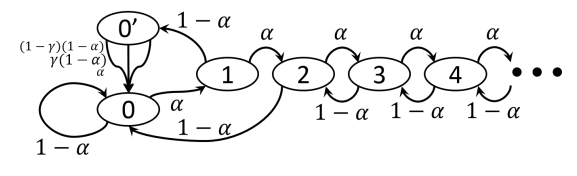
\includegraphics[width=8cm]{selfish_mining}
\centering
\caption{Selfish mining state machine with transition probabilities \cite{eyal2014majority}}
\label{fig:selfish_mining}
\end{figure}

Further research showed that more generalised selfish mining strategies lead to even more relative gain for the selfish miner \cite{nayak2016stubborn,sapirshtein2016optimal, gervais2015tampering, gervais2016security, bahack2013theoretical}.
\aju{Describe the \emph{relative gain} aspect here in one parapgraph before it is used in the above sentence. Maybe therefore first describe the term \emph{stale block rate}. Maybe start like that: One important metric in context of PoW Blockchains is the stale block rate. It ... }
The authors of \cite{nayak2016stubborn} provided a comprehensive description of the strategy space and also coined different names for the selfish mining variations:
\aju{Its better style to start a sentence with a word and not directly with a reference.}

\begin{itemize}
	\item \textbf{Lead stubborn}: 
	This mining strategy compromises the idea to cause as many block races as possible and to never overwrite the public chain with a longer chain.
	This strategy continuously tries to split the network to mine on different blocks and is therefore especially promising when the probability to win the block race is very high.
	\item \textbf{Equal-fork stubborn}: 
	The mining strategy equal-fork stubborn changes the selfish mining strategy just by one transition.
	In case the selfish miner finds a block during a block race, it does not publish his block to win the race but it also keeps this block undisclosed to secretly mine on this new tip of the chain.
\item \textbf{Trail stubborn}: 
The mining strategies based on trail stubbornness are reflecting the idea to even trail behind the public chain and to eventually catch up.
	Trail stubbornness is defined with an integer denoting how many blocks the strategy should allow the selfish miner to trail back.
\end{itemize}

The strategy space for a selfish miner is practically endless and combinations of the aforementioned strategies are possible and are leading to even more relative gain compared to honest miners \cite{nayak2016stubborn,sapirshtein2016optimal, gervais2015tampering, gervais2016security, bahack2013theoretical}.

\todo[inline]{extend to explain stale block rate}

To find the best strategy for a given mining power share $\alpha$ and connectivity $\gamma$ researchers used different methodologies.
\cite{eyal2014majority, sapirshtein2016optimal} used closed-source simulations which we cannot discuss here.
Other researchers used numeric simulations of paths in the state machine to find optimal selfish mining strategies \cite{gervais2015tampering, nayak2016stubborn}.
Lastly, \cite{sapirshtein2016optimal, gervais2016security} used MDPs based on a state machine to find strategies with the most relative gain.
The basic structure of the used state machines is for all publications the same, despite the MDP introduced by \cite{gervais2016security}.
They additionally they used in their MDP the so-called stale block rate which denotes the ratio between blocks from the consensus chain and stale blocks.
This metric accounts for the most important parameters of a blockchain protocol such as block sizes, block intervals, network delays, information propagation mechanisms and network configuration and can be seen as a general security parameter of a blockchain protocol.
The higher the stale block rate, the less secure the blockchain protocol \cite{gervais2016security}.

Besides using variations of the selfish mining strategies, the attack can also be combined with other attacks to achieve better results \cite{gervais2016security, sapirshtein2016optimal, nayak2016stubborn, gervais2015tampering}.
If the eclipse attack is used in combination with selfish mining the victim contributes its mining power to the private chain and hence, strengthens the position of the selfish miner \cite{nayak2016stubborn, gervais2016security}.
\cite{nayak2016stubborn} additionally shows that the eclipsed victim under certain circumstances can benefit from the attack and therefore has no incentive to stop the attack.
Another attack which can be used in combination with selfish mining is double-spending \cite{sapirshtein2016optimal, gervais2016security}.
Every time the selfish miner starts his selfish mining attack it can publish a transaction and include a conflicting transaction in his first secret block.
During the execution of the selfish mining attack, the payment receiver may accept the payment depending on his block confirmation time.
Now in the case of a successful selfish mining attempt, the adversary can overwrite the public chain, which additionally results in a successful double spending.
The operational costs of unsuccessful double-spending can be seen as low because the adversary still would get goods or a service in exchange for the transaction \cite{sapirshtein2016optimal, gervais2016security}.

Last but not least also the prevention of selfish mining is part of the current work in selfish mining research \cite{eyal2014majority, billah2015one, solat2016zeroblock, zhang2017publish}.
A backwards-compatible patch to mitigate selfish mining is uniform tie-breaking \cite{eyal2014majority}.
This means whenever a node receives two blocks of the same height it randomly select one of the blocks to mine on.
\cite{eyal2014majority} showed that this would raise the profit threshold to 25\% of the computational power and hence mitigating selfish mining.
The drawback of this proposed change is that it would increase the connectivity of badly connected attackers to almost 50\% with no actual effort for them.
Ethereum, the currently second largest cryptocurrency by market capitalization \cite{marketcap2017}, has implemented uniform tie-breaking as a countermeasure against selfish mining \cite{gervais2016security, unifromtiebreakingethereum}.
Another countermeasure foresees unforgeable timestamps to secure Bitcoin against selfish mining \cite{billah2015one}.
This countermeasure would make all pre-mined blocks of the selfish miner invalid after a certain amount of time.
The implementation of this patch would require random beacons and hence introduce complexity and a new attack vector \cite{billah2015one}.
\cite{zhang2017publish} proposes backwards-compatible countermeasure by neglecting blocks that are not published in time and allows incorporation of competing blocks in the chain similar to Ethereum's uncle blocks \cite{wood2014ethereum}.
This enables a new fork-resolving policy where a block always contributes to neither or both branches of the fork \cite{zhang2017publish}.
All of this mentioned countermeasures are not planned to be implemented or implemented in Bitcoin \cite{bitcoin, bitcoinbip}.
The countermeasures against selfish mining are forming an interesting research field but are not in the focus of this thesis.
Nevertheless, all of them would profit from an evaluation method introduced in the next chapter.


\chapter{Expected results}
The expected outcome of this thesis is a more accurate simulation of different selfish mining strategies and therefore a better understanding of the potential real world implications of such attacks.
The selfish mining strategies used in the thesis include:
\begin{itemize}
\item selfish mining \cite{eyal2014majority}
\item lead stubborn mining \cite{nayak2016stubborn}
\item trail stubborn mining \cite{nayak2016stubborn}
\item equal-fork stubborn mining \cite{nayak2016stubborn}
\end{itemize}

For the simulation, these strategies are combined with different distributions of computation power in the underlying peer-to-peer network.
The result of the simulations should show which strategy is the best strategy for a certain distribution of mining power and if the selfish mining increases the relative gain of the selfish miner compared to the normal, honest mining.
The simulation results should emphasise the recent work in the area of selfish mining and show that the current implementation of Bitcoin protocol is vulnerable against different selfish mining strategies.

The desired outcome of the thesis is supported with the following two research questions:

\begin{itemize}
	\item \textbf{RQ1:} Do the simulations of selfish mining with the proposed software solutions show an increase of the relative gain for the selfish miner compared to the normal, honest mining behaviour?

	\item \textbf{RQ2:} How does the obtained results of the simulation match the outcome of previous research in the area of selfish mining?
\end{itemize}


An additional outcome of the thesis is the simulation software.
The software should allow an accurate and deterministic simulation of the blockchain by using directly the reference implementation and a realistic network topology.
Hence, the simulation software could not only be used to simulate selfish mining attacks but could for example also be used to simulate other attacks or new protocol versions of Bitcoin. 
Since many other cryptocurrencies are derived from Bitcoin, they simulation software could be used also to simulate their behaviour and properties.


\chapter{Methodology and Approach}
First, the different strategies selfish, lead stubborn, trail stubborn and equal-fork stubborn mining from \cite{nayak2016stubborn} and \cite{eyal2014majority} need to be implemented.
This is achieved by implementing a proxy which eclipses a normal Bitcoin client from the other nodes in the network.
Now, if a block is found the proxy decides, depending on his selfish mining strategy, if a block should be transmitted from the eclipsed node to the rest of the network or vice versa.
The proxy design pattern makes it possible to implement the selfish mining strategies without altering the reference implementation of Bitcoin and is therefore preferred over an implementation directly in the Bitcoin client.

In the next step, a simulation program is implemented.
To be able to control when a certain node finds a block, all Bitcoin nodes should be executed in \textit{regtest} mode.
In this test mode, the real PoW-algorithm is disabled and every node accepts a command which lets the node create immediately a new block.
With this functionality, it is possible to define a block discovery series which basically reflects the computation power of each node.
The more blocks are found by a node the more simulated computation power the node has.
Additionally to the block generation, the simulation program should also control the network topology and hence the connectivity of each node.
For the simulation run, it is important that the connectivity of the nodes stays the same to make the results better comparable.
This should be achieved by setting the connections from the nodes by the simulation program itself which is in contrast to normal behaviour.
Normally Bitcoin nodes share their connections with other nodes over the Bitcoin protocol and try to improve the connectivity over time.

After the implementation of the selfish mining strategies and the simulation program, the mining strategies are simulated.
Different network topologies and distributions of computation power are used to compare the relative gain of the selfish mining strategies over the normal, honest mining.


\chapter{Simulation software}
The simulation software provides all needed functionalities to orchestrate a peer-to-peer network where the nodes are running the \textit{Bitcoin} reference implementation.
The whole simulation runs on a single host using the virtualisation software \textit{Docker}.
The software furthermore coordinates the block discovery in the network.
Based on a sequence defined in a configuration file the software sends commands to the nodes which are then generating valid blocks.
To be able to create blocks the nodes are executed in the \textit{regtest mode}, where the CPU-heavy proof-of-work is disabled, and the nodes are accepting a RPC-call from outside which lets them create a new block immediately.
After a simulation run, the software parses the logs produced by the nodes and based on them the software generates a report which displays the key metrics of the simulation.
\todo[inline]{go a little into the details what the rational behind this desgin was. eg. predefined sequence.}

The remaining of this chapter starts with the sub-chapter \ref{chap:tick}, where the general concept of a tick is introduced.
Afterwards in the chapter \ref{chap:config_files} the different configuration files are explained.
In the chapter \ref{chap:simulation} the whole procedure of a simulation with the three main steps preparation, execution and post-processing is explained.
Lastly, in the chapter \ref{chap:commands} the implemented commands to execute the simulation framework are listed.
  
\section{Tick}
\label{chap:tick}

A fundamental concept of the simulation software is a so-called tick.
A tick represents a small time span containing information about which nodes should find a new block in this tick.
Hence a tick forms an abstraction of a certain time span in the real time.
All blocks which should be generated in this time span are aggregated into the corresponding tick.
Since all blocks created in the same tick are considered to be created at the same time, a tick should never contain the information that one node creates multiple blocks.

For a simulation run, multiple ticks are generated forming a sequence of ticks.
This sequence is the simulation scenario for a particular simulation run.
The exact duration of a tick is defined on execution time of the simulation and determines the actual speed of the simulation.
The concept of a tick helps to have an upper bound for the simulation speed.
An upper bound of a certain sequence of ticks is reached when the execution time of at least one tick last longer than the tick duration itself.
In that case, the temporal succession of the block events is disturbed resulting in inaccurate or wrong results, and the simulation speed should be lowered.

\section{Configuration files}
\label{chap:config_files}

A simulation executed by the software needs to be configured with the configuration files \textit{nodes.csv}, \textit{network.csv} and \textit{ticks.csv}.
The configuration files are stored in the concise CSV format and on a specific location on the disk to be processed by the simulation software.
The usage of configuration files as input for a simulation provide the flexibility that they can be written manually or that they can be generated by a small script.
Also a combination of both is possible.
For example, a small script generates a needed configuration file.
Afterwards, the user can adjusted the configuration file by editing it and does not need to implemented a own script for the specific scenario, but does also no need to write the whole configuration file by hand.
Furthermore, the created configuration files can be copied to the output directory of a simulation run providing easy method to preserve all input parameters used for run.

The simulation software already implements for each configuration file a simple script which can be executed by the corresponding commands \textit{nodes} (chapter \ref{chap:nodes_command}), \textit{network} (chapter \ref{chap:network_command}) and \textit{ticks} (chapter \ref{chap:ticks_command}).

\subsection{\textit{nodes.csv}}

The \textit{nodes.csv} contains the configuration of every node which should be orchestrated by the simulation software.
Each row in the file reflects one node consisting of:
\begin{itemize}
	\item \textit{node\_type}: Either \textit{bitcoin} if the node is a normal node or \textit{selfish} if the node should act like a selfish node.
	\item \textit{share}: The computation power proportion of the node in the network.
	\item \textit{docker\_image}: The \textit{Docker} image to use for the node.
	\item \textit{latency}: The latency  of the node in the peer-to-peer network.
	The node will have this latency to all other nodes with the exact same latency.
	For other connections the two different latencies are added.
	Hence, two nodes, one node with 100 milliseconds of latency and one node with 50 milliseconds, will have 150 milliseconds of latency during the simulation.
	\item \textit{group}: Which group the node did belong to during the creation of the \textit{nodes.csv} by the script introduce in chapter \ref{chap:commands}.
	During the actual execution of the simulation this parameter is ignored.
\end{itemize}
 
\subsection{\textit{network.csv}}
The \textit{network.csv} reflects a connection matrix as shown in table \ref{tab:network_csv}.
The simulation software starts each node in a way that a node on the y-axis tries to establish an outgoing connection to another node on the x-axis whenever the corresponding value in the matrix is 1.

\begin{table}
  \centering
  \begin{tabular}{c|ccc}
    			& node a 	& node b	& node c	\\
    \hline
    node a		& 0			& 1         & 0         \\
    node b      & 0         & 0         & 1			\\
    node c      & 1         & 1			& 0         \\
  \end{tabular}
  \caption{An example \textit{network.csv} represented as table}
  \label{tab:network_csv}
\end{table}

\subsection{\textit{ticks.csv}}

The \textit{ticks.csv} contains all ticks which should be executed by the simulation software.
Each line represents a tick with no, one or multiple block events.
Hence the length of lines in a \textit{ticks.csv} varies depending on the number of block events in the corresponding tick.

\section{Simulation}
\label{chap:simulation}

The main functionality of the simulation software is to coordinate a simulation based on the configuration files.
The software uses therefore the high-level programming language \textit{Python} and the virtualisation software technology \textit{Docker}.
\textit{Python} is mainly used to handle the configuration files and to execute \textit{Docker} and other binaries whenever necessary automatically.
\textit{Docker} on the other side provides the needed capabilities to run the \textit{Bitcoin} reference implementation and other programs in virtual, lightweight containers on one single host.
These containers are using the functionalities of the same kernel in an isolated manner and hence they do not interfere each other as long as the host system provides enough resources to them.
The containers can also reuse the networking stack of the kernel, making possible to create a peer-to-peer network needed for the simulation.
Furthermore by using \textit{Docker} all containers use the system time of the host machine.
This is especially helpful for the aggregation of the log files of all different containers, because it assures that the timestamps in the log lines actually happened in exactly this order.
	
To execute a simulation the command \textit{simulate} (chapter \ref{chap:simulate_command}) can be used.
In that case the configuration files need to be available on disk.
The commands \textit{run} (chapter \ref{chap:run_command}) and \textit{multi-run} (chapter \ref{chap:multi_run_command}) provide another possibility to execute a simulation, creating all configuration files before starting the simulation. 

\begin{figure}[t]
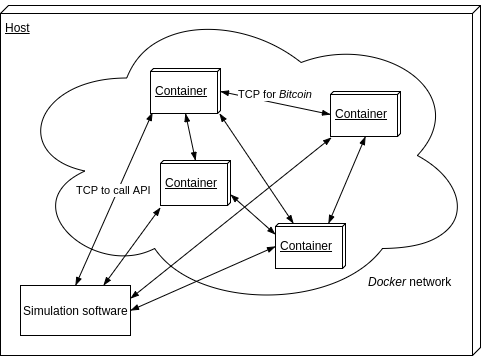
\includegraphics[width=8cm]{overview_setup}
\centering
\caption{Overview of the virtual peer-to-peer network}
\label{fig:overview}
\end{figure}

\subsection{Preparation}

The preparation phase is the first phase of a simulation run.
At the beginning, a simulation directory is created and all configuration files are copied into the new directory to assure reproducibility.
Subsequently, a virtual peer-to-peer network is assembled as depicted in figure \ref{fig:overview}.
Therefore firstly a \textit{Docker} network with the driver set to \textit{bridge} is created which under the hood configures a new network interface in the networking stack of the host machine.
This network interface is used by the \textit{Docker} containers to connect and communicate to other containers.
Afterwards based on the two configuration files \textit{nodes.csv} and \textit{networking.csv} the nodes are created as \textit{Docker} containers with \textit{bitcoind} set as command to be executed in the container.
Listing \ref{lst:docker_create} shows how \textit{Docker} is used to create a container, which executes \textit{bitcoind} on start-up.
In line 2 the unique IP of the container is set by using the \textit{-{}-ip} argument.
Line 3 shows the usage of a so-called \textit{Docker volume} to mount the folder \textit{data/run-10/node-5/} into the container's folder \textit{/data/regtest}.
By running \textit{bitcoind} in \textit{regtest mode} (line 6) and setting the data directory of \textit{bitcoind} to \textit{/data} (line 7) \textit{Bitcoin} persists all relevant data into \textit{/data/regtest}.
Hence all the data persisted by \textit{bitcoind} under \textit{/data/regtest} will actually be persisted under \textit{data/run-10/node-5/} on the host machine and is therefore still available after the destruction of the container.
In line 8 we define to which other nodes the node should connect to by specifying their IP.
By using the \textit{-connect} parameters the \textit{Bitcoin} reference implementation automatically stops to listen for incoming connections.
Since this is needed to accept incoming connections, it is re-enabled in line 9 by setting \textit{-listen} to 1.

Lastly, after all nodes are spawned, an RPC-connection to the \textit{Bitcoin} API running in each node is established by using the library \textit{python-bitcoinlib}.
These connections are later used to directly send commands to the nodes.

\begin{minipage}{\linewidth}
\begin{lstlisting}[caption=Simplified version of how a node is started with \textit{Docker} and \textit{bitcoind}, label={lst:docker_create}, basicstyle=\ttfamily, captionpos=b]
docker run
	--ip=240.1.0.5
	--volume data/run-10/node-5:/data/regtest
	bitcoind_image
		bitcoind
			-regtest
			-datadir=/data
			-connect=240.1.0.2 -connect=240.1.0.9
			-listen=1
\end{lstlisting}
\end{minipage}
	
\subsection{Execution}

In the execution phase the simulation software iterates over each tick from the \textit{ticks.csv}.
If a tick contains a block event, the framework calls \textit{generate} on the \textit{Bitcoin} API of the specific node to generate a new block.
Since all nodes are running in \textit{regtest mode} the proof-of-work is deactivated and the block can be created immediately.
Some ticks may contain multiple block events.
In this case the block events are executed one after another always waiting for the block hash to be returned by the nodes.
The sequential execution of the block events is preferred over a parallelisation, which would introduce a new source of uncontrollable indeterminism making the results harder to reproduce even on the same host.

A simulation run is always executed with a certain tick duration.
This tick duration specifies how long a tick should last in real time.
Therefore the simulation framework simply keeps track of the passed time during the execution of the block events and sleeps afterwards until the tick is over.
If the completion of the block events last longer then the tick duration, then the framework immediately starts with the next tick and tries to regain the lost time.
The case where the execution of block events last longer then the tick duration, should be a rare exception.
If this happens more frequent the simulation scenario is configure too fast, which likely creates inaccurate results as explained in chapter \ref{chap:tick}.
Thus, the defined scenario should be created with less block events per tick or a higher tick duration should be configured on simulation start.
The simulation software warns the user about the total amount of exception of this type in the final report.

During the execution of the ticks a thread separately collects information about the current CPU and memory usage.
For the CPU usage the thread queries periodically the \textit{/proc/stat} file which is showing how much time the CPU spent in a certain state. 
The collected snapshots can later be used to determine the actual utilization of the CPU by calculating the differences between the snapshots.
For the memory usage the thread reads periodically the \textit{MemAvailable} in \textit{/proc/meminfo} file.
This value provides a heuristic of the current available memory on the machine.

\subsection{Post-processing}

The post-processing phase is the last phase of a simulation run.
At the beginning of this phase the consensus chain, denoting the longest chain of blocks all nodes agree about, is calculated.
This is done by starting at block height one and asking each node for the hash of the block on this height in their longest chain.
If all nodes have a block at this height and the hashes of all blocks are the same, then all nodes reached consensus and the block is added to the consensus chain.
In the next step the height is increased by one and the previously described check is repeated.
If one node has no block at a certain height or the hashes of the blocks differ then the calculation of the consensus chain stops.

After the calculation of the consensus chain all \textit{Docker} nodes are stopped and removed.
Because a separate data directory was mounted on each node by using \textit{Docker volumes} all relevant data, especially the log files, are still available on the host machine after the deletion of the \textit{Docker} nodes.
In the next step lines of the logs from nodes and from the log file of the simulation framework are parsed to retrieve information about the simulation run.
These log line types are:

\begin{itemize}
   \item \textit{BlockGenerateLine}: Log line produced by a node when a new block is generated.
   \item \textit{BlockStatsLine}: A log line displaying various information like block size about a freshly generated block.
   \item \textit{UpdateTipLine}: Log line produced by a node whenever a block updates a tip of the chain.
   \item \textit{PeerLogicValidationLine}: Log line produced when the proof-of-work of a received compact block is checked.  
   \item \textit{BlockReconstructLine}: A log line created when a compact block was successfully reconstructed.
   \item \textit{BlockReceivedLine}: Log line created when node receives a normal block.
   \item \textit{TickLine}: A log line with information about an executed tick.
   \item \textit{BlockExceptionLine}: Log line created whenever the simulation framework was not able to successfully execute a block event.
   \item \textit{RPCExceptionEventLine}: Log line denoting an exception occurred while using the RPC-connection to a node.
\end{itemize}

The log lines \textit{BlockGenerateLine}, \textit{BlockStatsLine}, \textit{UpdateTipLine}, \textit{PeerLogicValidationLine}, \textit{BlockReconstructLine} and \textit{BlockReceivedLine} are all produced by nodes executing \textit{Bitcoin} where on the other hand \textit{TickLine}, \textit{BlockExceptionLine} and \textit{RPCExceptionEventLine} are created by the simulation software itself.
Furthermore, the \textit{BlockGenerateLine} log line was added especially for the simulation software to the \textit{Bitcoin} reference implementation.
Normally the reference implementation does not create a log line containing the block hash when it creates a new block.
To circumvent this fact, a log line was added to the reference implementation to persist the event of the block creation including a hash of the block.

The simulation software persists all parsed log lines into CSV files where each log line type gets its file.
Subsequently the \textit{preprocess.R} script prepares the CSV files for the final report creation.
When a simulation is executed a parameter can be passed which denotes how many ticks at the beginning and at the end should not be evaluated in the post-processing phase (\textit{skip\_ticks}).
The \textit{R} script then figures out when the first and the last tick to be evaluated occurred and tailors the log line types \textit{BlockGenerateLine} and \textit{BlockStatsLine} respectively.
All other types do not need to be tailored because they either are used to calculate some combined statistics like the block propagation time or because the statistics of these types are still calculated over the whole simulation duration like the memory usage.
The \textit{skip\_ticks} parameter allows the user to discard ticks which may created distorted data.
Right after the start it is likely that the nodes behave differently because the execute some initializing routines or run faster because they just started up.
At the end of the simulation run it makes sense to ignore some ticks because blocks created at the end of the simulation would distort the analysis of the simulation.
Those blocks probably propagate faster, because right after them no other competing blocks are created.
Another problem could be that the simulation frameworks already starts to shut down the peer-to-peer network even though some blocks are still transmitted to other nodes.
How many ticks should be omitted depends on the simulation scenario and the right amount is difficult to determine.
An additional mitigation is to extend the overall simulation, which would reduce the influence of the distorted data from the first and last ticks.

Additionally to omitting some ticks, the \textit{preprocess.R} script sorts all CSV files according to the timestamp of the log line.
This is necessary because the parsing of the log files is implemented in a multi-threading manner and thus the ordering from the original log files is lost.

After all CSV files are created the simulation frameworks generates a report by executing a \textit{R Markdown} file.
The final report contains:
\begin{itemize}
	\item general information about the simulation like the start and end time
	\item specifications and settings of the host machine used in the simulation
	\item all input arguments passed to the simulation
	\item summary about planned, executed and parsed block events
	\item overview of the duration of each phase of the simulation
	\item chart visualizing CPU and memory utilization
	\item chart showing the duration of a tick over time
	\item charts and information about blocks created during the simulation
	\item charts and information about exceptions happened during the simulation
\end{itemize}

Where most of the information and charts are just simple representations of the data present in the CSV files, the stale block rate and the propagation time of blocks needs to be calculated in the report.
\todo[inline]{Do not undersell ;)}
	The stale block rate and propagation time of blocks needs to be calculated in the report.
todo[inline]{The term stale block rate should be explained in the State-of-the-Art section when talking about the other simulations - this is a key metric that is important and it should be clear why - maybe also cite Eyals Bitcoin NG}

The stale rate, describing how many blocks did not end up in the longest chain, is calculated by checking each created block against the consensus chain determined previously by simply merging the \textit{BlockGenerateLine} log lines with the consensus chain.
The propagation time of blocks is calculated with \textit{R} as shown in listing \ref{lst:propagation_time}.
First the \textit{BlockGenerateLine} log lines are merged with the lines describing the event of receiving a block, namely	\textit{UpdateTipLine}, \textit{PeerLogicValidationLine}, \textit{BlockReconstructLine} and \textit{BlockReceivedLine} creating a new data frame.
Since for example \textit{UpdateTipLine} is also logged by the node which created the block in line 5 all these elements are filtered out of the data frame.
Afterwards the data set is grouped by the block hash and the name of the node (line 7).
By filtering out the element with the lowest timestamp, the data frame now represent the points in time when a node heard first about a certain block.
Lastly the propagation time is calculated by subtracting the timestamp of the \textit{BlockGenerateLine} log line from the timestamp of the receiving log lines.

\begin{minipage}{\linewidth}
\begin{lstlisting}[caption=Calculation of propagation time with \textit{R}, label={lst:propagation_time}, basicstyle=\ttfamily, captionpos=b]
log_lines <- merge(log_lines_receiving_block, block_generate,
		   by = 'hash')

log_lines %>%
  filter(as.character(node.x) != as.character(node.y)) %>%
  select(-node.y, node = node.x) %>%
  group_by(hash, node) %>%
  filter(which.min(timestamp.x)==row_number()) %>%
  mutate(propagation_time = timestamp.x - timestamp.y)
\end{lstlisting}
\end{minipage}
 
\subsection{Multi-runs}

When the simulation software is executed with the \textit{multi-run} command (chapter \ref{chap:multi_run_command}) multiple simulations are conducted depending on the passed input arguments.
After each simulation the created CSV files of the simulation are copied by the simulation software into an own directory.
Once the last simulation finishes the software aggregates all copied CSV files into single CSV files for each log line type.
Subsequently the \textit{R Markdown} file, which also is used to create the final report of a single  simulation, is executed to create a report comparing all simulation runs.
 
\section{Commands}
\label{chap:commands}

The simulation software exposes six commands to the user.
Three of this commands are creating configuration files necessary for the execution of a simulation. One command, the \textit{simulate} command, executes a simulation based on these configuration files.
The other two commands, \textit{run} and \textit{multi-run}, are aggregations of the before mentioned commands.

\subsection{\textit{nodes} command} \label{chap:nodes_command}

The \textit{nodes} command can be executed with so-called node groups (eg. \textit{node\_group\_a}) as input parameters.
A node group represents a group with a certain amount of nodes sharing the same node type, Docker image and latency.
Alongside these attributes a node group specifies a certain share of the computational power in the network.
On execution the simulation framework parses all passed node groups and checks if the shares defined for each group are summing up to a total of 100\%.
In that case, the framework persists the nodes of each group in a file called \textit{node.csv}, where the share of the computational power of the group is equally distributed over all members of the respective group.

\subsection{\textit{network} command} \label{chap:network_command}

When the simulation software gets executed with the \textit{network} command it reads a \textit{node.csv}, which needs to be available, to determine all planned nodes.
Based on an additional connectivity parameter (\textit{connectivity}), which defines with how many nodes a node should be connected, the simulation software creates a matrix reflecting connections between two nodes.
The Bitcoin reference implementation itself does not differentiate between established incoming or outgoing connection, hence it suffices to define one connection in the connection matrix if two nodes should be connected.
The connection matrix is afterwards persisted in the configuration file \textit{network.csv}.

\subsection{\textit{ticks} command} \label{chap:ticks_command}

The \textit{ticks} command can be used to create the configuration file \textit{ticks.csv}, which contains the ticks to be executed.
When executing the \textit{ticks} command the simulation software accepts one parameter denoting the amount of ticks to create (\textit{amount\_of\_ticks}) and one parameter about how many blocks per tick should be generated by the nodes (\textit{blocks\_per\_tick}).
Additionally the simulation software reads the \textit{nodes.csv}, which needs to be available, to determine all planned nodes and their computational share (\textit{share}).
Afterwards the software parametrises for each node an exponential distribution as shown in \ref{eq:exponential} with $\lambda = blocks\_per\_tick \cdot share$.
From this exponential distribution sufficient samples are drawn, which are denoting points in time when a specific nodes should find a block.
With this time series at hand the ticks are created by starting with the 1st tick.
For every point in time lower then the number of current tick a block event for the respective node is added to the tick and the point in time is removed from the time series.
This procedure is repeated for every tick until reaching \textit{amount\_of\_ticks}.
For example if we calculated the five samples 0.4, 0.8, 2.3, 4.1 and 5.8 for an arbitrary node A.
Furthermore the desired \textit{amount\_of\_ticks} would be 5.
Then we would get five ticks, where in the 1st tick are two block events for node A, and in the 3rd tick  and 5th tick one each.
The 2nd and the 4th tick would stay empty. After calculating all ticks, the ticks are persisted in the \textit{ticks.csv}.

 \begin{equation} \label{eq:exponential}
f(x; \lambda) = \begin{cases*}
        1 - \exp(-\lambda x) & x  $\geq$ 0, \\
        0                                    &  x < 0
        \end{cases*}
\end{equation}

\subsection{\textit{simulate} command} \label{chap:simulate_command}

On execution of the \textit{simulate} command the simulation software starts a simulation based on the configuration files \textit{nodes.csv}, \textit{network.csv} and \textit{ticks.csv}.
All these files need to be available and furthermore, the duration of ticks (\textit{tick\_duration}) and the amount of ticks which events should not be evaluated (\textit{skip\_ticks}) are parsed as input arguments.
Afterwards the simulation software executes the simulation as described in section \ref{chap:simulation}.

\subsection{\textit{run} command} \label{chap:run_command}

When the simulation software is started with the \textit{run} command basically the commands \textit{nodes}, \textit{network}, \textit{ticks} and \textit{simulate} are executed in exactly this order.
It is possible to pass all desired input arguments to the specific commands, but since the simulation is started right after the creation of the configuration files, it is not possible to change those files before the simulation.

\begin{figure}[t]
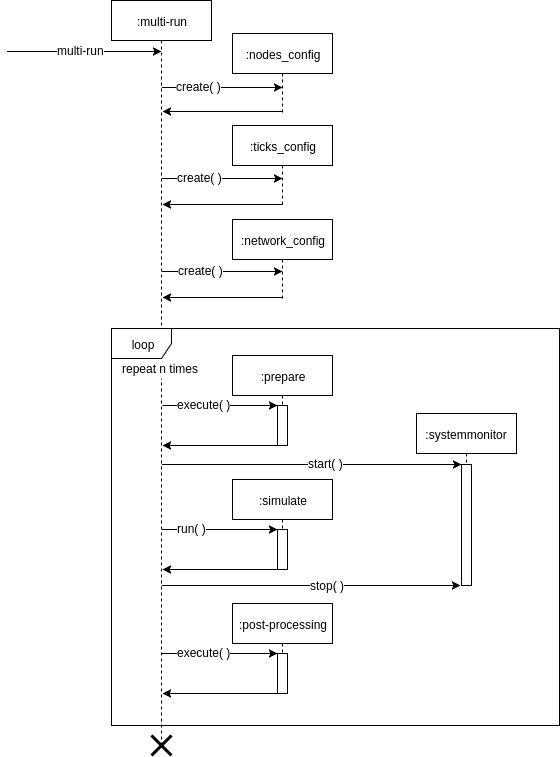
\includegraphics[width=8cm]{flow_chart_multi_run}
\centering
\caption{Sequence diagram of the \textit{multi-run} command}
\label{fig:flow_chart_multi_run}
\end{figure}

\subsection{\textit{multi-run} command} \label{chap:multi_run_command}

The \textit{multi-run} command accepts an input parameter denoting how often a run should be repeated ($repeat$).
The simulation software then creates all configuration files using the passed input arguments and subsequently executes the simulation $repeat$ times using the same configuration files as depicted in figure \ref{fig:flow_chart_multi_run}.

\todo[inline]{You could also add some notes on ZFS and alignment - this is relevant for long time storage of simulation data. This is perfectly valid since this chapter is dealing with engineering questions anyway.}


\chapter{Evaluation of simulation software}
The simulation of eight different selfish mining strategies with five distinct distributions of computational power provides a reasonable outcome to argue the two research questions of the thesis.

\section{RQ1}

\textit{Do the simulations of selfish mining with the proposed software solutions show an increase of the total and relative gain for the selfish miner compared to the normal, honest mining behaviour?}

The simulation showed that the relative share of mining rewards obtained with selfish mining is higher compared to the honest mining if the miner has over 40\% of mining power and conducts a satisfactory selfish mining strategy.
To the satisfactory strategies, all strategies expect the combination lead stubborn and equal-fork stubborn (\textit{L, F}) and selfish mining with all three modifications (\textit{L, F T\textsubscript{1}}) can be counted.
The curves of the six good-performing strategies depicted in figure \ref{fig:accepted_blocks_selfish} show all a similar behaviour where their relative gain increases non-linearly with a higher computational share.
Out of these six strategies, the most promising strategies are normal selfish mining (\textit{S}) and equal-fork stubbornness (\textit{F}).
When these two strategies are applied, the selfish miner can create 49.1\%/50\% of the blocks of the longest chain even though its share of the mining power is only 45\%.

In all cases where the selfish miner has a low share of computational power, the results of the simulation show that the selfish mining does not increase the relative gain.
For example, when the selfish miner has 15\% of the mining power in the network only about 5\% of its blocks end up in the longest chain.
Even if the selfish miner has 37.5\% share of the computational power the most advantageously strategy (\textit{S}) only creates 32.4\% blocks of the longest chain.
The worst performing mining strategy in the scenario where the selfish miner has 37.5\% is the strategy with all three modifications (\textit{L, F, T\textsubscript{1}}) generating only 22.7\% of the accepted blocks.

Concluding it can be said that with the defined simulation scenario and the proposed software solutions only for a very high computational share an increase of the relative gain could be observed.
For all scenarios where the selfish miner has less than 40\% percent, the miner would earn relatively more by behaving honestly.

\section{RQ2}

\textit{How do the obtained results of the simulation match the outcome of previous research in the area of selfish mining?}

When comparing the outcome from the simulations with recent studies, it first needs to be considered that with the introduced simulation framework the outcome of the block races cannot be defined directly, as it is the case in previously used types of simulation.
Instead, the block races happen naturally during the execution of a scenario.
With the used simulation scenario and implementation of the selfish proxy, it is likely that the parameter $\gamma$, denoting if an honest node extends the private chain during a block race, is almost zero.
This assumption is based on the configured network topology and the implementation of the selfish proxy.
In the scenario, a fully connected network topology is used where each connection has the same latency.
Hence, when a node finds a block, it sends the block to all nodes directly.
Then it is unlikely that the selfish node can advertise its block faster to other nodes using the same connections before the honest nodes have already adopted to the new public tip.
The implementation of the selfish proxy further worsens the position of the selfish miner when trying to match a competing block during a block race.
The proxy which eclipses the private node does not implement the fast block propagation mechanism \textit{compact blocks}.
Instead, the proxy uses the standard but slower block propagation technique to receive and send blocks.
Thus, the proxy receives and sends blocks slower than the rest of the network.

Assuming that the probability of the selfish miner to win a block race is very low, the attained results match the outcome of previous research.
In figure \ref{fig:eyal_results} the red line shows the relative revenue of the selfish miner conducting normal selfish mining when it is not able to win any block race \cite{eyal2014majority}.
The curve shows the same concave course as in figure \ref{fig:accepted_blocks_selfish} underlining that with an increase of the computational share the efficiency of the selfish mining is amplified.
Moreover, the selfish miner achieved more relative revenue compare to the honest miner with about 36\% of the mining power, similar to the slightly worse results of 40\% showed in chapter \ref{chap:results}.
Comparable outcomes for the selfish mining without any modification were produced in other recent research \cite{nayak2016stubborn, sapirshtein2016optimal}.

\begin{figure}[t]
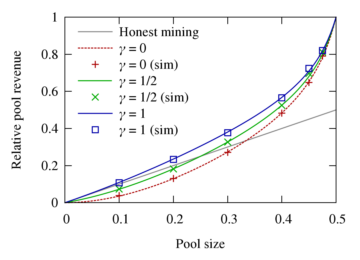
\includegraphics[width=8cm]{eyal_results}
\centering
\caption{Results obtained by \cite{eyal2014majority} with normal selfish mining}
\label{fig:eyal_results}
\end{figure}

In figure \ref{fig:nayak_results_1} optimal selfish mining strategies including stubborn modifications from the research of \cite{nayak2016stubborn} are shown.
In the case, where the selfish miner loses all block races, the honest behaviour is the most profitable strategy until a computational share of 34\% is reached.
Afterwards, the most advantageous mining strategy is trail stubbornness (\textit{T\textsubscript{1}}) up to a computational share of 45\%.
From 45\% to 50\% the dominant strategy is trail stubborn in combination with equal-fork stubborn (\textit{T\textsubscript{1}, F}), but in many cases, the best strategy is not clear signalised by the black dots in the graphic.
The results of the optimal stubborn mining strategy by \cite{nayak2016stubborn} slightly differ to the outcome of the simulation from chapter \ref{chap:results}.
In the proposed simulation the best performing strategies were the normal selfish mining (\textit{S}) and equal-fork stubborn mining (\textit{F}) with trail stubbornness combined with equal-fork stubbornness (\textit{T\textsubscript{1}, F}) and trail stubbornness (\textit{T\textsubscript{1}}) being only the third and fourth most satisfactory strategy.

\cite{nayak2016stubborn} does not propose the actual ranking of different selfish strategies regarding their performance for a specific $\gamma$ but provides a comparison of the relative gain obtained by selfish mining and selfish mining with stubborn modifications.
On the assumption that $\gamma$ is zero, the relative gain achieved by using stubborn modifications over selfish mining is very low as shown in figure \ref{fig:nayak_results_2}.
Thus, also in the research of \cite{nayak2016stubborn}, the normal selfish mining forms a viable strategy comparable to the results obtained in the previous chapters.
Furthermore, figure \ref{fig:nayak_results_1} showed that between 45\% and 50\% the best strategy is not always known denoted by the black dots.
From that concludes, that in the case where all block races are won by the honest network, the optimal strategy is not identifiable, similar to the outcome from the proposed simulations where the four best strategies were 3\% apart.

\begin{figure}[t]
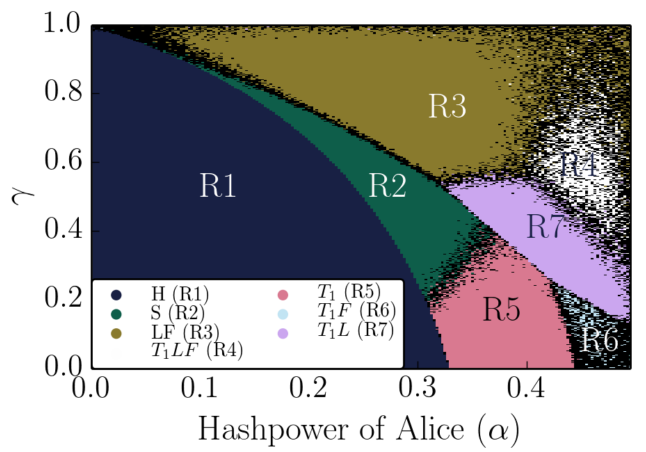
\includegraphics[width=8cm]{nayak_results_1}
\centering
\caption{Optimal stubborn mining strategies retrieved by \cite{nayak2016stubborn}}
\label{fig:nayak_results_1}
\end{figure}

Summarising the obtained simulations results are comparable to recent research even though the outcome of the simulation was slightly worse than results from previous research.
Regarding the best performing selfish mining strategies also the research of \cite{nayak2016stubborn} showed that differences in the case where $\gamma$ equals zero are subtle.
Nevertheless, both studies showed similar good performing selfish mining strategies.

\begin{figure}[t]
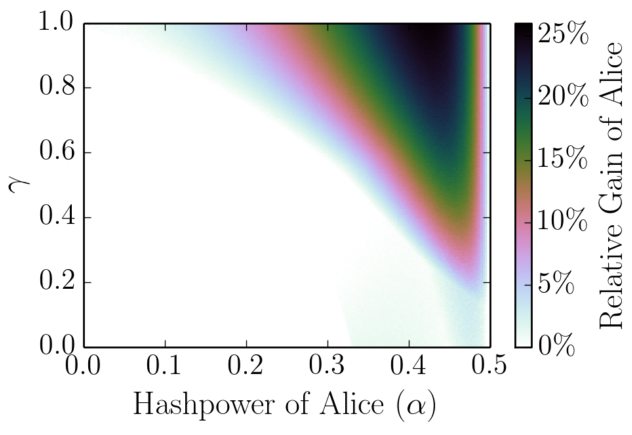
\includegraphics[width=8cm]{nayak_results_2}
\centering
\caption{Selfish mining compared to optimal stubborn mining strategies by \cite{nayak2016stubborn}}
\label{fig:nayak_results_2}
\end{figure}

\section{Profitability}

As previously evaluated selfish mining can increase the relative gain of the misbehaving miner, but the results of the simulations show further that the absolute amount of accepted blocks is lower as shown in figure \ref{fig:accepted_blocks_selfish}.
Hence, the selfish miner is earning less mining rewards even though its relative revenue is increasing.
The loss of profit is possible because the stale block rate increases during selfish mining, and thus, fewer blocks end up in the longest chain.
To still profit from the attack the miner would need to wait for the difficulty adjustment.
After the difficulty adjustment, the nodes in the network can find more blocks and hence, also the selfish miner can create more blocks.
Since selfish mining was never observed for such a long time and no research was conducted in this area, it is not clear if such a long attack would be successful \cite{nayak2016stubborn}.
\aju{Basically this needs to be stated somewhere earlier - either state-of-the-art or earlier in this chapter}


\chapter{Selfish proxy}
The selfish proxy is a node in the peer-to-peer network which performs selfish mining in collaboration with a connected, eclipsed Bitcoin node.
Together the two nodes are forming a selfish miner as shown in figure \ref{fig:selfish_proxy}.
The proxy implements parts of the Bitcoin communication protocol and requests all blocks created either by the honest network or by the eclipsed node.
With the retrieved blocks the selfish proxy recreates the chain locally and whenever the public or the private chain changes the node executes the configured selfish mining algorithm.
Depending on the outcome of the selfish mining algorithm the proxy afterwards relays blocks to the other part of the network.
With this withholding method, the selfish proxy can mimic different selfish mining strategies without creating a single block.

\section{Network}

The selfish proxy is a normal member of the peer-to-peer network and is also executed as a \textit{Docker} container.
During the simulation run, the proxy mimics the behaviour of a normal Bitcoin node.
In figure \ref{fig:selfish_proxy} a possible network topology with a selfish proxy is depicted.
The nodes on the left side are forming the honest, public network working together on the public chain.
The two nodes on the right side are forming the selfish miner where the proxy abuses the private chain build by the eclipsed node to execute a particular selfish mining strategy.
In the current implementation, the selfish proxy can only eclipse one single node.
In the case where the proxy could eclipse multiple nodes to build a private chain, the selfish proxy could also be used as a stand-alone man-in-the-middle attacking tool eclipsing a larger amount of nodes.

The topology of the peer-to-peer network in a simulation run is solely established by the simulation framework.
First, the software starts the selfish proxy which then just listens for new incoming connections.
Afterwards, the normal Bitcoin nodes are started with the respective \textit{-connect} parameters set.
If such a normal node has the IP of the selfish proxy set in a \textit{-connect} parameter, then the Bitcoin node simply connects to the listening proxy.
The proxy accepts the connection and behaves like a normal Bitcoin node during the whole simulation run by obeying the Bitcoin communication protocol.

\begin{figure}
	\centering
    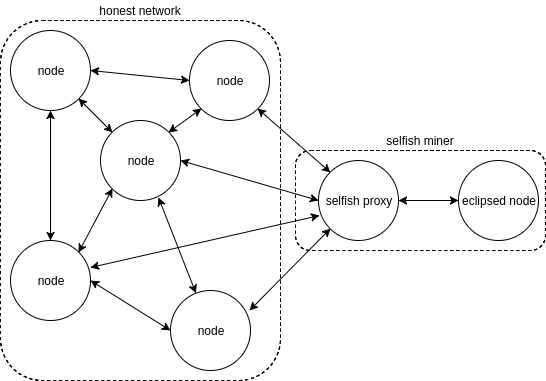
\includegraphics[width=10cm]{selfish_proxy}
    \caption{Selfish proxy eclipsing a normal node}
    \label{fig:selfish_proxy}
\end{figure}

The implementation of all network related functionalities of the selfish proxy is based on the two open-source libraries \textit{pycoin} \cite{pycoin} and \textit{python-bitcoinlib} \cite{python-bitcoinlib}.
The library \textit{pycoin} provides simple networking utilities to connect to other Bitcoin nodes and to manage those connections. 
The \textit{python-bitcoinlib} library, on the other hand, implements functionalities to serialise and de-serialise Bitcoin network messages.

\section{Chain}

The selfish proxy continuously collects all blocks and block headers sent by the connected peers and reassembles the whole chain locally.
To execute the selfish mining algorithm efficiently the proxy needs to retrieve updates of the private and public chain as fast as possible.
Therefore the proxy uses solely block headers to update the chain despite using whole blocks.
The block headers which contain all necessary information to update the chain can be retrieved faster than the full block because they are just a part of the block and hence smaller.
Furthermore, it is secure for the proxy to trust in the validity of the block header since all other nodes in the network are assumed to behave honestly in our simulation and hence are sending only valid block headers.

When the selfish proxy tries to update the chain with a so far unknown block header, it simply looks at the hash of the previous block stored in the block header.
If the previous block hash is in the chain, the newly received block header is appended to the chain.
On a programmatic level, the proxy uses for that a one-way linked list with the possibility to navigate to the previous block.
In the case the block header has no direct ancestor in the current chain, the header gets preserved as an orphan block.
All orphan blocks are checked on every successful insertion of a block if they now can be added to the chain.

Alongside the information stored in the block, the proxy also keeps track of the block origin and a boolean variable called \textit{transfer\_allowed}. 
The block origin is a simple enumeration if the block was received from the honest network or from the eclipsed node and hence does not change over time.
The \textit{transfer\_allowed} variable determines if the transfer of a block is allowed and is initially always set to \textit{False}.
Depending on the selfish mining strategy the block may be relayed to the other nodes at some later point in time changing the boolean to \textit{True}.
These two variables are stored to be able to distinguish between the public chain, the current longest chain known to the honest network and the private chain, the current longest chain known to the eclipsed node.
For example, to determine the current private chain all blocks originated by the eclipsed node and all blocks with \textit{transfer\_allowed} set to \textit{True} are used.
The two views of the chain are essential for the selfish mining algorithm to decide which action to take and hence when to relay which block to the other side of the network.

\begin{figure}
	\centering
    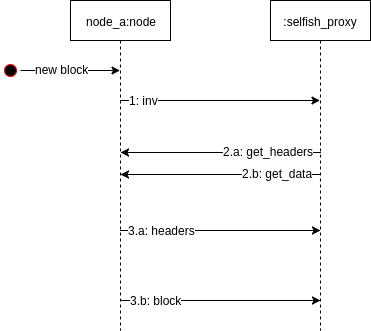
\includegraphics[width=7cm]{receive_block}
    \caption{Selfish proxy receiving a block from another node}
    \label{fig:receive_block}
\end{figure}

\section{Receiving blocks}
\label{chap:receiving_blocks}

An essential capability of the selfish proxy is to retrieve blocks and block headers from its peers.
Figure \ref{fig:receive_block} depicts the communication flow between an arbitrary node called \textit{node\_a} and the selfish proxy which wants to retrieve the information of a new block.
Firstly \textit{node\_a} either finds a new block itself or retrieves a new block from some other node in the network.
Then, adhering to the Bitcoin protocol, the node sends an \textit{inv} message (1) containing the hash of the block to its peers including the proxy.
The proxy subsequently checks if it already requested the block from another node or even has the block in the own local chain.
In this two cases, the proxy would just ignore the received hash, and the communication flow would end.
If the block hash is unknown, the proxy sends a \textit{get\_headers} (2.a) message and a \textit{get\_data} (2.b) message to the \textit{node\_a} as pictured in figure \ref{fig:receive_block}.

The \textit{get\_headers} message (2.a) sent by the proxy is composed with an array called block locator hashes and is used to retrieve all block headers after the known block hashes denoted in the array.
To create the array the proxy uses either the private or the public chain depending if \textit{node\_a} is the eclipsed node or a node of the honest network.
The proxy adds then the highest, 2nd, 4th, 8th and 16th highest blocks of the selected chain to the array.
If the chain does not provide all needed bocks, then only the available blocks are added to the block locator array.
\textit{Node\_a}, after it received the \textit{get\_headers}, will search the block hashes from the block locator array in its own longest chain starting with the highest block.
Once a block hash matches a block in the longest chain of \textit{node\_a}, \textit{node\_a} collects all block headers after the matched block in a \textit{headers} message and sends the message back to the proxy (3.a).
In the normal case the proxy trails just one block behind the highest block known by \textit{node\_a}, hence the headers message will contain only one single block header.
In the usual cases, the proxy actually felt more than one block behind and \textit{node\_a} will send multiple block headers back to the proxy.
Since the proxy only needs block headers to update the chain, it can immediately update with the received headers the whole chain to the newest tip known tho the \textit{node\_a}.

The \textit{get\_data} message (2.b) sent by the proxy just contains the block hash of the desired block.
As soon as the \textit{node\_a} receives the request for the block, it will return the full block in a \textit{block} message (3.b) to the node.
The request for the whole block lasts typically longer than the request for the newest block headers with the \textit{get\_headers} message as it is pictured in figure \ref{fig:receive_block}.
The proxy request the full block containing all information solely to be able to respond to \textit{get\_data} request by other nodes when it advertises the block on later point in time.

\begin{figure}
	\centering
    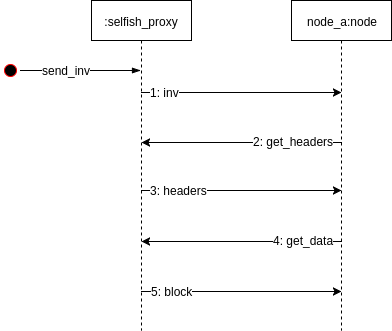
\includegraphics[width=7.5cm]{send_block}
    \caption{Selfish proxy sending a block to another node}
    \label{fig:send_block}
\end{figure}

\section{Sending blocks}
\label{chap:sending_blocks}

After the execution of the selfish mining algorithm, the proxy may want to send a block to the opposite origin of the block.
Figure \ref{fig:send_block} shows the communication flow between an arbitrary \textit{node\_a} and the selfish proxy which intends to relay a block.
The proxy therefore firstly sends the block hash as \textit{inv} message (1) to the \textit{node\_a}.
The \textit{node\_a} after receiving the \textit{inv} message will then reply with a \textit{get\_headers} message (2) because it has not seen the withheld block so far.
The \textit{get\_headers} message contains, similar to the \textit{get\_headers} build by the proxy when it receives a block, known block hashes by \textit{node\_a}.
The proxy then selects either the private or the public chain depending if \textit{node\_a} is the eclipsed node or a node of the honest network.
In the case that there is no unique, longest chain the selfish proxy prefers the chain where the origin of the highest block is the eclipsed node to promote the blocks of the eclipsed node.
Subsequently, the proxy iterates over the selected chain until a block hash from the locator array send by the \textit{node\_a} matches.
The proxy then returns all headers of the blocks after the matched block until the highest block composed in a \textit{headers} message (3).
Afterwards, the \textit{node\_a} will iterate over the received headers and request all missing blocks.
In the usual case, \textit{node\_a} will just lack one block which the node will simply request by sending a \textit{get\_data} message (4) to the proxy.
The selfish proxy replies to this message then by sending a \textit{block} message (5) containing the full block.
Since the selfish mining algorithm already processes the block header before the whole block is available, it could be the case that a block requested by a node is not yet available.
In this case, the proxy defers the reply to the node until it receives the entire block from another node.

\begin{figure}[t]
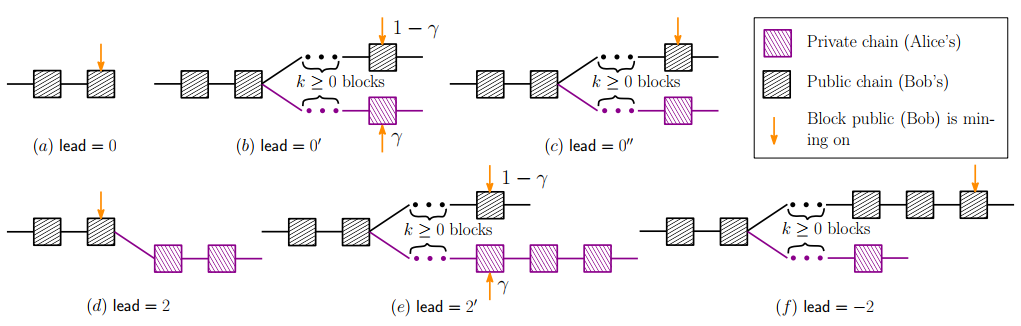
\includegraphics[width=15cm]{private_lead}
\centering
\caption{Different possible leads of the private chain \cite{nayak2016stubborn}}
\label{fig:private_lead}
\end{figure}

\section{Selfish mining}

The selfish proxy executes selfish mining in collaboration with an eclipsed node which is only connected to the proxy as shown in figure \ref{fig:selfish_proxy}.
During the simulation, the proxy monitors the honest network which works on the public chain and the eclipsed node which works on the private chain and performs selfish mining by withholding the blocks created by both sides.

\subsection{Private lead}

Every time a block header is inserted in the chain the proxy checks if either the public or private chain was altered.
In the case that one of these two chains changed the proxy executes the configured selfish mining algorithm.
To easier track the changes between the two chains an integer variable called private lead is used which describes the distance between the two tips of the chain as shown in figure \ref{fig:private_lead}.
A positive lead \textit{n} denotes an advantage of \textit{n} blocks of the private chain over the chain of the honest network.
Conversely, a negative lead \textit{n} stands for a \textit{n} block lag of the eclipsed node over the public chain.
Furthermore, there exist positive leads annotated with an apostrophe denoting that at the height of the public chain a block race happens.
In this block race, the possibility that the private chain is extended to the height of the public chain is $\gamma$ and the probability that the public chain gets extended is $1 - \gamma$.
Lastly, a private lead of zero can be annotated with two apostrophes expressing that both chains have the same height but everyone is mining on his own chain.

\subsection{Actions}

The execution of the algorithm outputs one of the four possible actions \textit{adopt}, \textit{override}, \textit{match} and \textit{wait} equivalent defined in the work of \cite{sapirshtein2016optimal}.
An action describes which blocks should be advertised and relayed to the other side of the network at a given point in time:

\begin{itemize}
	\item \textbf{Adopt}: 
	The action \textit{adopt} means that the selfish miner adopts the chain of the honest network. 
	This is a typical action if the private lead is zero and the honest network finds a new block. 
	Then it can be sensitive to just adopt to this new block.
	To execute the \textit{adopt} action the selfish proxy relays the public chain to the eclipsed node by advertising unknown, public blocks.
	\item \textbf{Override}:
	The \textit{override} action is only possible if the private lead is greater then zero after the insertion of the new block header.
	In this case, the selfish proxy can override the public chain by sending out the private blocks mined by the eclipse node.
	Hence, when the proxy executes the \textit{override} action, it sends all private blocks including the first block strictly higher than the public chain.
	If there are even higher private blocks, the selfish proxy keeps them back for further selfish mining.
	\item \textbf{Match}:
	The \textit{match} action is only feasible if the private lead previous the insertion of the block header was greater than zero and the origin of the block is the honest network.
	In this case, the selfish proxy can advertise the private block at the same height to the honest network creating a block race.
	After the execution of the \textit{match} action, the resulting private lead is annotated with an apostrophe to denote the block race.
	\item \textbf{Wait}:
	If the selfish algorithm outputs the \textit{wait} action, then the proxy does simply nothing and waits for the next block which changes either the private or the public chain.
\end{itemize}

\begin{figure}[t]
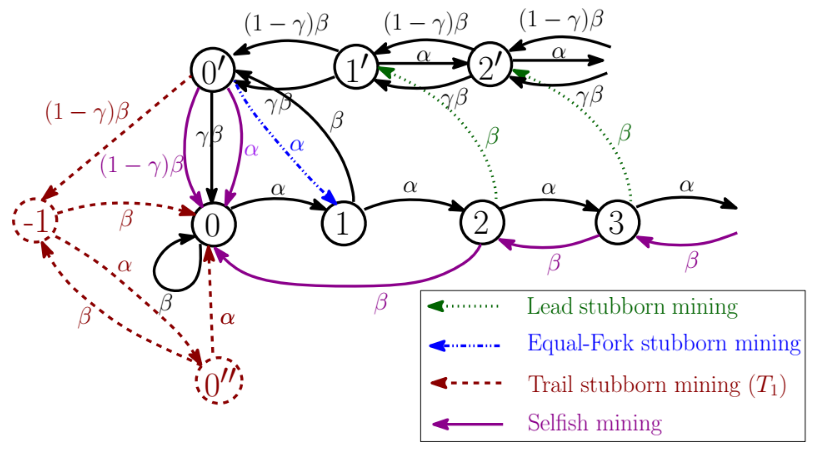
\includegraphics[width=10cm]{stubborn_mining}
\centering
\caption{Categorization of different mining strategies \cite{nayak2016stubborn}}
\label{fig:stubborn_mining}
\end{figure}

\subsection{Strategies}

The selfish mining strategies are defining which action the algorithm implemented in the proxy should execute after a new block was found in the network.
All strategies implemented in the proxy are based on the selfish mining strategy described by \cite{eyal2014majority} (abbreviated with \textit{H}) and can be modified with the three modifications lead (\textit{L}), equal-fork (\textit{F}) and trail stubborn (\textit{T}) by \cite{nayak2016stubborn}.
Figure \ref{fig:stubborn_mining} shows all strategies as a state machine where the label of the states stands for the private lead.
The labels $\alpha$ and $\beta$ used in the transitions are describing the probability that either the eclipsed node or the honest network finds a block.
The variable $\gamma$ represents the likelihood that the part of the honest network which mines on the private chain finds a block.

In the normal selfish mining strategy, two possible cases can occur in state \textit{0}.
If the honest network finds a block, then the selfish miner immediately adopts to the public chain and hence remains in the state \textit{0}.
In the other case where the selfish miner finds a block, the state 1 is reached because the selfish miner does not share the block with the honest network.
The same happens if the selfish miner finds more blocks.
Then the selfish miner simple does not share his blocks advancing to state \textit{2} and onwards.
In state \textit{1} the selfish miner has a private lead of one block.
If then the honest network honest network finds a block the selfish miner immediately releases the private block and starts a block race.
Any node in the honest block either chooses the private-public or the public block to mine on top depending which block it sees first.
The block race is dissolved after any node in the network finds a block.
If the honest network finds a block, then the selfish miner adopts to the new tip.
In the other case where the selfish miner finds a block, it immediately sends out the block to win the race.
In both cases, the state \textit{0} is reached again.
Lastly, if the private lead is two and the honest network finds a block then the selfish miner immediately publishes the two blocks.
This overrides the newly created block by the honest network, and the state \textit{0} is reached.

As introduced by \cite{nayak2016stubborn} the selfish mining strategy can be modified as follows:

\begin{itemize}
	\item \textbf{Lead stubborn mining (\textit{L})}:
	In lead stubborn mining, the selfish miner tries to cause as many block races as possible.
	So whenever the private chain is longer than the public chain, and the honest network finds a block the selfish miner releases the competing block with the same high causing a block race.
	This behaviour is also applied in state \textit{2} where the selfish miner overwrites typically the block appended to the public chain by publishing two blocks.
	In lead stubborn mining, the selfish miner only releases the competing block an starts a block race denoted with the state \textit{2'}.
	This strategy is promising when $\gamma$ is high implying that whenever a block race occurs, it is likely that the honest network finds a block on published block of the selfish miner. 
	Hence, the honest network unwillingly helps the selfish miner to succeed the private chain during the block race.
	\item \textbf{Equal-fork stubborn mining (\textit{F})}:
	The equal-fork stubborn mining strategy changes the behaviour of the selfish miner during a block race in state \textit{0'}.
	Usually, the selfish miner would use the created block to overwrite the public chain hence winning the block race.
	Using the equal-fork stubborn strategy, the miner keeps the block back which leads to state \textit{1} and the honest network remains mining on two different tips of the chain.
	Thus the strategy compromises the idea to keep the honest network split over two chains as long as possible.
	\item \textbf{Trail stubborn mining (\textit{T})}:
	In trail stubborn mining, the selfish miner allows the private chain to even trail behind the public chain.
	If the block race in state \textit{0'} is won by the honest network, the selfish miner does not adopt the public chain and trails back leading into the state \textit{-1}.
	In the case that the selfish miner can catch up by creating a new block the state \textit{0''} where both chains have the same length.
	The trail stubborn strategy finally pays off when the selfish miner finds another block and can override the public chain with the private chain.
	Trail stubbornness is parametrised with an integer \textit{n} determining how many blocks the private chain is allowed to trail behind the public chain.
	If this threshold is reached the selfish miner dismisses his private chain and adopts to the public chain by reaching again state \textit{0}.
\end{itemize}

The modifications of the selfish mining strategy can lead to even more gain for the selfish miner depending on the actual computational share and the parameter $\gamma$.
Furthermore, the strategies can be combined and since the trail stubbornness can be parametrised the build an infinite strategy space.

\subsection{Algorithm}

The selfish mining strategies and its modifications are implemented in selfish proxy by a simple algorithm using normal control flow structures.
Since the selfish proxy does not have a holistic overview of when a node finds a block, it only can try to apply selfish mining whenever the public or private chain changes locally after the insertion of a new block header.
The algorithm mimics the behaviour shown in the state diagram from figure \ref{fig:stubborn_mining} by looking at the private lead before the insertion of the block header and the origin of the inserted block header.
For example, if the private lead before the insertion of the block header was one and the block header was appended to the public chain.
This would correspond to the state \textit{1} and the outgoing transition $\beta$ which leads in the state diagram to the state \textit{0'} denoting a block race.
The selfish mining algorithm must now assure that this state is also reached in the simulated network by starting a block race.
Thus the algorithm needs to execute the \textit{match} action by publishing the private block to the honest network.

Listing \ref{lst:algo} shows a part of the algorithm, namely the part where the private lead before the insertion is 0, and an action to be executed is searched.
Hence, this part of the algorithm reflects the states 0, 0' and 0'' of the state machine pictured in figure \ref{fig:selfish_mining}.
In the lines 2 to 6, the state 0 is treated by simply looking at the origin of the last block.
If the block was mined by the honest network, then the proxy just adopts to the public chain.
In the other case, the block was found by the eclipsed node, and the proxy just waits for the next block to be discovered.

\begin{minipage}{\linewidth}
\begin{lstlisting}[caption=Part of the selfish mining algorithm where private lead is zero, label={lst:algo}, basicstyle=\ttfamily, captionpos=b]
if private_lead == 0:
    if length_private == 0:
        if last_block_origin is BlockOrigin.public:
            return Action.adopt
        else:
            return Action.wait
    else:
        if last_block_origin is BlockOrigin.public:
            if self.trail_stubborn < 0:
                return Action.wait
            else:
                return Action.adopt
        else:
            if self.active and self.equal_fork_stubborn:
                return Action.wait
            else:
                return Action.override
\end{lstlisting}
\end{minipage}

The lines 7 to 17 are covering the 0' and 0'' states.
In the case the last block was found by the honest network, the proxy adopts to the public chain except the algorithm was configured with trail stubbornness.
Then the proxy waits and hopes to catch up with the public chain at a later point (line 10).
The other case, implemented from line 7 to 17, reflects the fact when the block is found by the eclipsed node.
Then normally the proxy would override the chain by sending the respective private blocks to the honest network.
An exception to this is when currently a block race is happening, and the algorithm is configured with equal-fork stubbornness.
In that case, the selfish algorithm currently has set the variable \textit{active} to \textit{True} and applies equal-fork stubbornness by executing the \textit{wait} action.

\subsection{Configuration}

The selfish proxy started with any configuration executes the standard selfish mining strategy with no modifications.
On execution time the three modifications lead, equal-fork and trail stubborn mining can be configured by using input arguments:

\begin{itemize}
	\item \textit{lead\_stubborn}:
	A boolean input argument determining if lead stubbornness should be used. 
	\item \textit{equal\_fork\_stubborn}:
	A boolean input argument defining if equal-fork stubbornness should be applied or not.
	\item \textit{trail\_stubborn}:
	Used with an integer specifying how much the selfish proxy should trail back.
\end{itemize}

\aju{The typesetting of this page looks strange - only one sentence on the last page and then one empty page - but this can be neglected}


\chapter{Simulation of selfish mining strategies}
With the introduced software solutions, the simulation software and the selfish proxy, it is now possible to analyse selfish mining and its impact on the relative gain of the selfish miner.
For the simulation, the scenario described in chapter 45 is adapted.
One of the twenty nodes is eclipsed with the selfish proxy forming a selfish miner.
To obtain a comprehensive overview of the impact of selfish mining the selfish miners conducts various combinations of selfish mining strategies.
Additionally, different distributions of the computation power between the nodes and the selfish miner are applied.

\section{Selfish mining scenarios}

As strategies, the standard selfish mining strategy and the three modifications lead stubborn, equal-fork stubborn and trail stubborn mining are put into action.
The used trail-stubborn strategy is parametrised with 1 meaning that the selfish miner will at the maximum trail one block behind the public chain.
Hence, the at least trail stubborn strategy is executed in the different scenarios.
Since the modifications of the selfish mining strategies can be combined a total of eight different selfish mining strategies are executed during the simulation.

For the distribution of computation power, five different settings are used where the selfish miner receives either 15\%, 22.5\%, 30\%, 37.5\% or 45\% of the computation power.
The rest of the computation power in each scenario is distributed equally over all remaining, honest nodes.
The five used shares are each 7.5\% apart covering sensitive shares of the computation share.
All possible scenarios where the selfish miner would receive more than 50\% are omitted because in that cases for the selfish miner it would be more efficient to launch the so-called 51\%-attack copping all mining rewards \cite{nakamoto2008bitcoin, clarkresearch, tschorsch2016bitcoin}.
Additionally, the scenario with a share of 7.5\% is discarded because it is very likely that in that case, selfish mining has no advantages as already shown in previous studies \cite{eyal2014majority, sapirshtein2016optimal, nayak2016stubborn}.

With eight different mining strategies and five different distributions of computation power, a total of 40 different scenarios are obtained.
Listing \ref{lst:simulation_cmd} shows how a specific scenario is started with the simulation software.
In this particular scenario, the selfish miner receives 30\% of the computation power (line 4), and the rest of the network consisting of 19 nodes gets with 70\% the rest of the mining power (line 3).
As shown in line 5 the selfish mining strategy in this simulation run is modified with equal-fork and trail stubbornness.
These arguments are passed by the simulation software to the selfish proxy when it gets created.
Furthermore, it can be seen in line 5 that the strategy modification trail stubborn is set to 1.
From line 6 to 8 the scenario is configured with the same blocks per tick rate, amount of ticks and tick duration as in the reference scenario described in chapter 45.

\begin{minipage}{\linewidth}
\begin{lstlisting}[caption=Command to execute a particular selfish mining scenario, label={lst:simulation_cmd}, basicstyle=\ttfamily, captionpos=b]
python3 simcoin.py multi-run 
	--repeat 3 
	--group-a bitcoin 19 0.7 25 simcoin/patched:v2 
	--group-b selfish 1 0.3 0 simcoin/proxy:v1 
	--selfish-args '--equal-fork-stubborn --trail-stubborn 1' 
	--blocks-per-tick 0.0333333333333333 
	--amount-of-ticks 60480 
	--tick-duration 0.1
\end{lstlisting}
\end{minipage}

\section{Simulation}

The previously defined selfish mining scenarios are executed on a \textit{x86 Linux} host machine with 16 virtualised cores and 57.718 GB of memory, the same machine used to examine the deterministic behaviour of the simulation software in chapter 45.
Each scenario gets executed three times by using the \textit{multi-run} command as shown in line 1 and 2 in the listing \ref{lst:simulation_cmd}.
To extract a particular metric from the multiple executions of a scenario, the simulation with the median stale block rate is used.
Since the simulation software can not behave perfectly deterministic due its architecture, the median provides a robust method against possible outliers and hence, more accurate results are achieved.

\section{Results}

\afterpage{
    \begin{landscape}
        \tiny
        \centering
  		\begin{tabular}{ccccccccc}
    		\toprule
			strategy & share & blocks honest & blocks selfish & stale blocks honest & stale blocks selfish & share selfish & share stale selfish & stale block rate \\
			\midrule
                        H & 0.150 & 1560.6 & 275.4 & 79.050 & 13.950 & 0.15000000 & 0.1500000 & 0.04821151 \\
            H & 0.225 & 1422.9 & 413.1 & 72.075 & 20.925 & 0.22500000 & 0.2250000 & 0.04821151 \\
            H & 0.300 & 1285.2 & 550.8 & 65.100 & 27.900 & 0.30000000 & 0.3000000 & 0.04821151 \\
            H & 0.375 & 1147.5 & 688.5 & 58.125 & 34.875 & 0.37500000 & 0.3750000 & 0.04821151 \\
            H & 0.450 & 1009.8 & 826.2 & 51.150 & 41.850 & 0.45000000 & 0.4500000 & 0.04821151 \\
            S & 0.150 & 1536 & 78 & 108 & 193 & 0.04832714 & 0.6411960 & 0.15718016 \\
            S & 0.225 & 1350 & 166 & 149 & 237 & 0.10949868 & 0.6139896 & 0.20294427 \\
            S & 0.300 & 1116 & 328 & 232 & 231 & 0.22714681 & 0.4989201 & 0.24278972 \\
            S & 0.375 & 919 & 442 & 299 & 271 & 0.32476120 & 0.4754386 & 0.29518384 \\
            S & 0.450 & 624 & 601 & 446 & 249 & 0.49061224 & 0.3582734 & 0.36197917 \\
            L & 0.150 & 1538 & 79 & 106 & 192 & 0.04885591 & 0.6442953 & 0.15561358 \\
            L & 0.225 & 1350 & 160 & 149 & 243 & 0.10596026 & 0.6198980 & 0.20609884 \\
            L & 0.300 & 1126 & 301 & 222 & 258 & 0.21093203 & 0.5375000 & 0.25170425 \\
            L & 0.375 & 931 & 415 & 287 & 298 & 0.30832095 & 0.5094017 & 0.30295184 \\
            L & 0.450 & 648 & 538 & 422 & 312 & 0.45362563 & 0.4250681 & 0.38229167 \\
            F & 0.150 & 1542 & 70 & 102 & 201 & 0.04342432 & 0.6633663 & 0.15822454 \\
            F & 0.225 & 1356 & 152 & 143 & 251 & 0.10079576 & 0.6370558 & 0.20715037 \\
            F & 0.300 & 1120 & 314 & 228 & 245 & 0.21896792 & 0.5179704 & 0.24803356 \\
            F & 0.375 & 921 & 417 & 297 & 296 & 0.31165919 & 0.4991568 & 0.30709477 \\
            F & 0.450 & 597 & 597 & 473 & 253 & 0.50000000 & 0.3484848 & 0.37812500 \\
            T\textsubscript{1} & 0.150 & 1534 & 81 & 110 & 190 & 0.05015480 & 0.6333333 & 0.15665796 \\
            T\textsubscript{1} & 0.225 & 1350 & 163 & 149 & 240 & 0.10773298 & 0.6169666 & 0.20452156 \\
            T\textsubscript{1} & 0.300 & 1119 & 325 & 229 & 234 & 0.22506925 & 0.5053996 & 0.24278972 \\
            T\textsubscript{1} & 0.375 & 921 & 441 & 297 & 272 & 0.32378855 & 0.4780316 & 0.29466598 \\
            T\textsubscript{1} & 0.450 & 648 & 575 & 422 & 275 & 0.47015536 & 0.3945481 & 0.36302083 \\
            L, F & 0.150 & 1543 & 65 & 101 & 206 & 0.04042289 & 0.6710098 & 0.16031332 \\
            L, F & 0.225 & 1362 & 136 & 137 & 267 & 0.09078772 & 0.6608911 & 0.21240799 \\
            L, F & 0.300 & 1160 & 254 & 188 & 305 & 0.17963225 & 0.6186613 & 0.25852124 \\
            L, F & 0.375 & 981 & 306 & 237 & 407 & 0.23776224 & 0.6319876 & 0.33350596 \\
            L, F & 0.450 & 733 & 375 & 337 & 475 & 0.33844765 & 0.5849754 & 0.42291667 \\
            L, T\textsubscript{1} & 0.150 & 1537 & 77 & 107 & 194 & 0.04770756 & 0.6445183 & 0.15718016 \\
            L, T\textsubscript{1} & 0.225 & 1353 & 153 & 146 & 250 & 0.10159363 & 0.6313131 & 0.20820189 \\
            L, T\textsubscript{1} & 0.300 & 1131 & 302 & 217 & 257 & 0.21074669 & 0.5421941 & 0.24855794 \\
            L, T\textsubscript{1} & 0.375 & 922 & 420 & 296 & 293 & 0.31296572 & 0.4974533 & 0.30502330 \\
            L, T\textsubscript{1} & 0.450 & 648 & 537 & 422 & 313 & 0.45316456 & 0.4258503 & 0.38281250 \\
            F, T\textsubscript{1} & 0.150 & 1540 & 68 & 104 & 203 & 0.04228856 & 0.6612378 & 0.16031332 \\
            F, T\textsubscript{1} & 0.225 & 1353 & 151 & 146 & 252 & 0.10039894 & 0.6331658 & 0.20925342 \\
            F, T\textsubscript{1} & 0.300 & 1119 & 317 & 229 & 242 & 0.22075209 & 0.5138004 & 0.24698479 \\
            F, T\textsubscript{1} & 0.375 & 911 & 429 & 307 & 284 & 0.32014925 & 0.4805415 & 0.30605904 \\
            F, T\textsubscript{1} & 0.450 & 613 & 581 & 457 & 269 & 0.48659966 & 0.3705234 & 0.37812500 \\
            L, F, T\textsubscript{1} & 0.150 & 1545 & 62 & 99 & 209 & 0.03858121 & 0.6785714 & 0.16083551 \\
            L, F, T\textsubscript{1} & 0.225 & 1358 & 138 & 141 & 265 & 0.09224599 & 0.6527094 & 0.21345952 \\
            L, F, T\textsubscript{1} & 0.300 & 1160 & 255 & 188 & 304 & 0.18021201 & 0.6178862 & 0.25799685 \\
            L, F, T\textsubscript{1} & 0.375 & 1000 & 294 & 218 & 419 & 0.22720247 & 0.6577708 & 0.32988089 \\
            L, F, T\textsubscript{1} & 0.450 & 720 & 389 & 350 & 461 & 0.35076646 & 0.5684340 & 0.42239583 \\
    		\bottomrule
  		\end{tabular}
  		\captionof{table}{Results of the 40 simulations with the additional honest behaviour \textit{H}}
  		\label{tab:simulation_results}
	\end{landscape}
}

The results of the 40 simulations are shown in table \ref{tab:simulation_results}.
In the first column, the different selfish mining strategies and its combinations are listed in abbreviated form.
The second column reflects the  computational share of the selfish miner during each specific simulation.
The two columns \textit{blocks honest} and \textit{blocks selfish} contain the number of blocks from each party which ended up in the longest chain.
The following two columns reflect the number of stale blocks for the honest network and the selfish miner.
The columns \textit{share selfish} and \textit{share stale selfish} are derived from the previous columns and describe the relative proportion of accepted and stale blocks for the selfish miner.
Lastly, in the ninth column, the overall stale block rate of each simulation run is stated.
Additionally, to the 40 results, the simulation with the median stale block rate from the evaluation of the simulation software in chapter 45 is added with the abbreviation \textit{H}.
Since in that simulation the computational share was always distributed evenly amongst all nodes the result of the simulation is multiplied by the corresponding share for each defined distribution of computation power.

\begin{figure}[t]
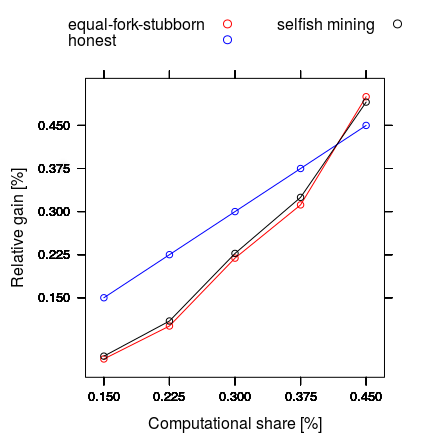
\includegraphics[width=12cm]{relative_block_share}
\centering
\caption{Relative revenue of the selfish miner}
\label{fig:relative_block_share}
\end{figure}

In figure \ref{fig:relative_block_share} the relative revenue, given a particular computation share and selfish mining strategy, is shown.
The graph shows that the two strategies selfish mining with \textit{lead stubborn, equal-fork stubborn} (\textit{L, F}) and selfish mining with all three modifications (\textit{L, F, T\textsubscript{1}}) are the worst performing strategies.
The relative share of accepted blocks of the two strategies stays clearly under the relative proportion which could be obtained by behaving honestly.
Also with an increase of the computational power the efficiency of the two selfish strategies is not amplified and the curve shows a linear progression.
The other six, better performing strategies are all exhibiting a similar behaviour.
The performance of these strategies is intensified with the augmentation of the computational share underlined by a concave curve.
Overall all selfish mining strategies are performing poorly and only with a computational share of about 40\% the six better performing strategies can retain a more significant share than the share obtained behaving honestly.
In table \ref{tab:relative_share_45} the relative  revenue share of the selfish miner with 45\% of computation power is shown.
The best performing strategies are equal-fork stubbornness (\textit{F}) and normal selfish mining (\textit{S}) followed by trail stubborn mining modified with equal-fork stubbornness \textit{F, T\textsubscript{1}} and the strategy trail stubborn (\textit{T\textsubscript{1}}).
These four strategies achieve almost similar results and are only 3\% apart.

\begin{table}
  \centering
  \begin{tabular}{cccc}
    \toprule
    strategy & share selfish & rank & difference to best\\
    \midrule
    F & 50\% & 1 & - \\
    S & 49.1\% & 2 & 0.9\% \\
    F, T\textsubscript{1} & 48.7\% & 3 & 1.3\% \\
    T\textsubscript{1} & 47\% & 4 & 3\% \\
    L & 45.4\% & 5 & 4.6\% \\
    L, T\textsubscript{1} & 45.3\% & 6 & 4.7\% \\
    H & 45\% & 7 & 5\% \\
    L, F, T\textsubscript{1} & 35.1\% & 8 & 14.9\% \\
    L, F & 33.8\% & 9 & 16.2\% \\
    \bottomrule
  \end{tabular}
  \caption{Relative share of selfish miner with 45\% of computational share}
  \label{tab:relative_share_45}
\end{table}

\begin{figure}[t]
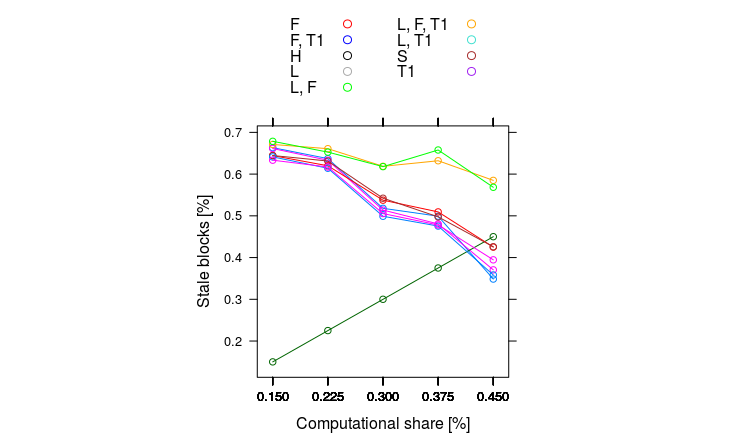
\includegraphics[width=12cm]{stale_blocks}
\centering
\caption{Share of stale blocks created by the selfish miner}
\label{fig:stale_blocks}
\end{figure}

Figure \ref{fig:stale_blocks} shows the share of stale blocks found by the selfish miner.
In the honest case, the share of created stale blocks increases linearly with the computational share.
Contrary to the line showing the honest behaviour proceed the lines depicting the different selfish mining strategies.
Especially if the computational share is low, over 60\% of the stale blocks of the network are created by the selfish miner.
With an increasing share of computational power, the share of stale blocks declines significantly, except the two strategies lead stubborn combined with equal-fork stubborn (\textit{L, F}) and selfish mining modified with all stubborn variations (\textit{L, F, T\textsubscript{1}}) which remain on the same level.
Additionally, the figure shows that only with a very high amount of computational share the selfish strategies are achieving better results than the normal, honest behaviour.

\begin{figure}[t]
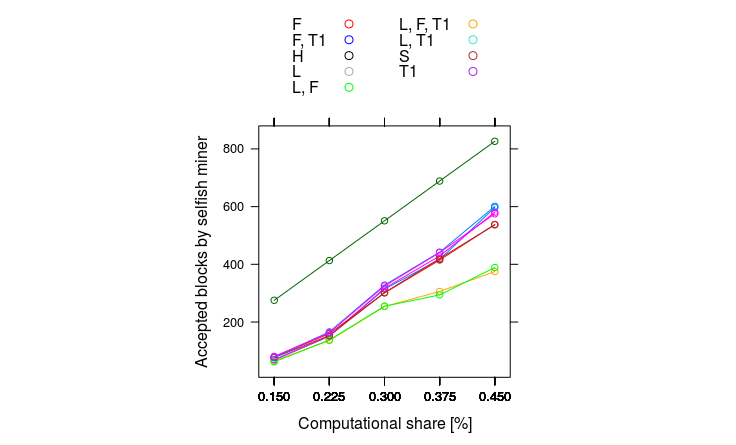
\includegraphics[width=12cm]{accepted_blocks_selfish}
\centering
\caption{Blocks created by the selfish miner and accepted in the longest chain}
\label{fig:accepted_blocks_selfish}
\end{figure}

The total amount of accepted blocks by the selfish miner, given a particular strategy and computational share, is shown in figure \ref{fig:accepted_blocks_selfish}.
The graph shows again the gap between the two bad performing strategies and the six other strategies which work slightly better.
Additionally, it can be seen that the absolute amount of accepted blocks during the execution of selfish mining is significantly lower than the number of blocks accepted when the nodes behave honestly.
Hence, in the short-run, all selfish mining strategies are yielding less mining rewards for the selfish miner than the normal, honest behaviour.

\begin{figure}[t]
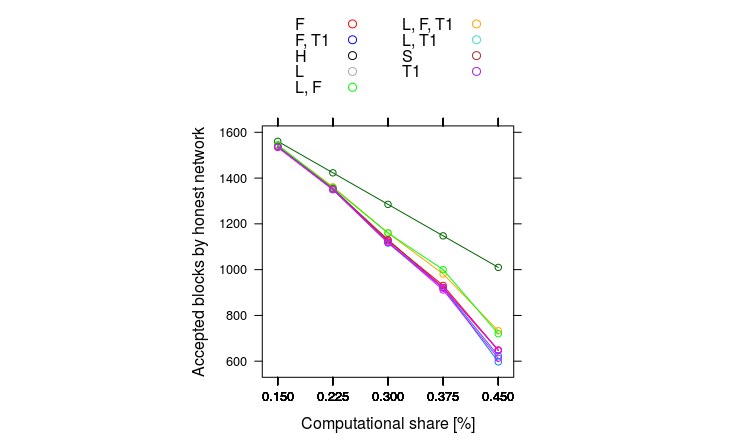
\includegraphics[width=12cm]{accepted_blocks_honest}
\centering
\caption{Blocks created by the honest network and accepted in the longest chain}
\label{fig:accepted_blocks_honest}
\end{figure}

The honest network also creates less accepted blocks during a selfish mining attack as shown in figure \ref{fig:accepted_blocks_honest}.
Since the selfish mining strategies are functioning better with an increasing computational share of the selfish miner, the gap between the case where all nodes behave honestly and the case where one node conducts selfish mining even increases.
The performance differences between the selfish mining strategies can also be seen in this figure.

\begin{figure}[t]
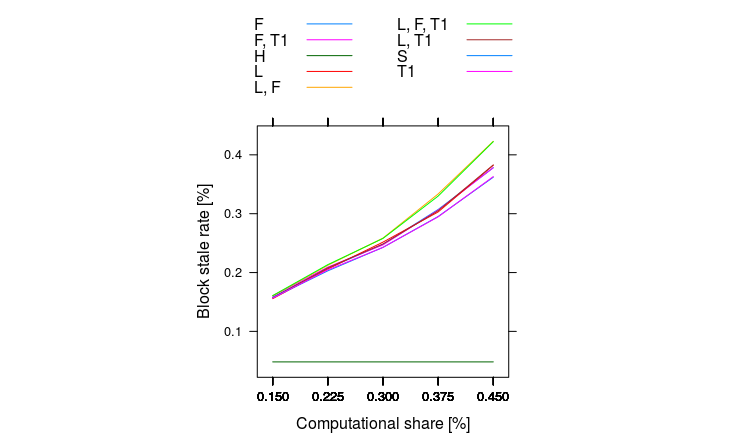
\includegraphics[width=12cm]{stale_rate}
\centering
\caption{Stale block rate}
\label{fig:stale_rate}
\end{figure}

Lastly, in figure \ref{fig:stale_rate} the relative amount of stale blocks in the network during the simulations is shown.
If all nodes behave honestly, the stale block rate is 4.821\% as measured during the evaluation of the simulation software.
In the case that a node conducts a selfish mining strategy the stale block rate is significantly higher and increases further if the computational power of the selfish miner is augmented.
Furthermore, the gap between the two worst performing selfish strategies and the other strategies can be observed.
If a node conducts lead stubbornness combined with equal-fork stubbornness (\textit{L, F}) or selfish mining with all three modifications (\textit{L, F, T\textsubscript{1}}), there are even more stale blocks in the network.

Similar as during the evaluation of the deterministic behaviour of the simulation software in chapter 45, also during the execution of the selfish mining scenarios the utilisation of the CPU and the memory of the host machine stayed under 10\% as shown in figure \ref{fig:selfish_simulations_cpu} and figure \ref{fig:selfish_simulations_memory}.
Thus, the specifications of the host machine did not restrict the simulations in any way.

\begin{figure}[t]
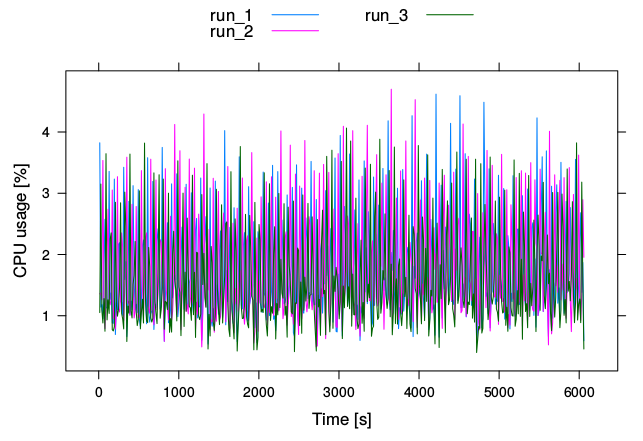
\includegraphics[width=8cm]{selfish_simulations_cpu}
\centering
\caption{CPU usage during the triple execution of a simulation scenario}
\label{fig:selfish_simulations_cpu}
\end{figure}

\begin{figure}[t]
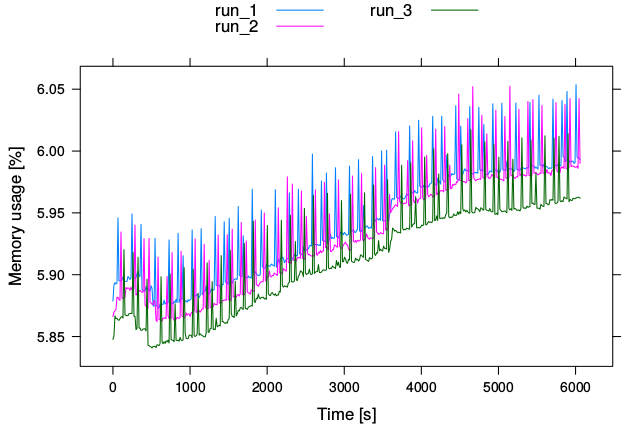
\includegraphics[width=8cm]{selfish_simulations_memory}
\centering
\caption{Memory usage during the triple execution of a simulation scenario}
\label{fig:selfish_simulations_memory}
\end{figure}


\chapter{Discussion}
\section{Installation}



\chapter{Further research}
\section{Installation}



% Remove following line for the final thesis.
%% intro.tex
%% Copyright (C) 2014-2016 by Thomas Auzinger <thomas@auzinger.name>
%
% This work may be distributed and/or modified under the
% conditions of the LaTeX Project Public License, either version 1.3
% of this license or (at your option) any later version.
% The latest version of this license is in
%   http://www.latex-project.org/lppl.txt
% and version 1.3 or later is part of all distributions of LaTeX
% version 2005/12/01 or later.
%
% This work has the LPPL maintenance status `maintained'.
%
% The Current Maintainer of this work is Thomas Auzinger.
%
% This work consists of the files vutinfth.dtx and vutinfth.ins
% and the derived file vutinfth.cls.
% This work also consists of the file intro.tex.


\newacronym{ctan}{CTAN}{Comprehensive TeX Archive Network}
\newacronym{faq}{FAQ}{Frequently Asked Questions}
\newacronym{pdf}{PDF}{Portable Document Format}
\newacronym{svn}{SVN}{Subversion}
\newacronym{wysiwyg}{WYSIWYG}{What You See Is What You Get}

\newglossaryentry{texteditor}
{
  name={editor},
  description={A text editor is a type of program used for editing plain text files.}
}

\chapter{Introduction to \LaTeX}

Since \LaTeX\ is widely used in academia and industry, there exists a plethora of freely accessible introductions to the language.
Reading through the guide at \url{https://en.wikibooks.org/wiki/LaTeX} serves as a comprehensive overview for most of the functionality and is highly recommended before starting with a thesis in \LaTeX.

\section{Installation}

A full \LaTeX\ distribution\index{distribution} consists of not only of the binaries that convert the source files to the typeset documents, but also of a wide range of packages and their documentation.
Depending on the operating system, different implementations are available as shown in Table~\ref{tab:distrib}.
\textbf{Due to the large amount of packages that are in everyday use and due to their high interdependence, it is paramount to keep the installed distribution\index{distribution} up to date.}
Otherwise, obscure errors and tedious debugging ensue.

\begin{table}
  \centering
  \begin{tabular}{cccc}
    \toprule
    Distribution & Unix         & Windows      & MacOS        \\
    \midrule
    TeX Live     & \textbf{yes} & yes          & (yes)        \\
    MacTeX       & no           & no           & \textbf{yes} \\
    MikTeX       & no           & \textbf{yes} & no           \\
    \bottomrule
  \end{tabular}
  \caption{\TeX/\LaTeX\ distributions for different operating systems. Recomended choice in \textbf{bold}.}
  \label{tab:distrib} % \label has to be placed AFTER \caption to produce correct cross-references.
\end{table}

\section{Editors}

A multitude of \TeX\ \glspl{texteditor} are available differing in their editing models, their supported operating systems and their feature sets.
A comprehensive overview of \glspl{texteditor} can be found at the Wikipedia page  \url{https://en.wikipedia.org/wiki/Comparison_of_TeX_editors}.
TeXstudio (\url{http://texstudio.sourceforge.net/}) is recommended.
Most editors support the scrolling the typeset preview document to a location in the source document by \verb|Ctrl| clicking the location in the source document.

\section{Compilation}

Modern editors usually provide the compilation programs to generate \gls{pdf} documents and for most \LaTeX\ source files, this is sufficient.
More advanced \LaTeX\ functionality, such as glossaries and bibliographies, needs additional compilation steps, however.
It is also possible that errors in the compilation process invalidate intermediate files and force subsequent compilation runs to fail.
It is advisable to delete intermediate files (\verb|.aux|, \verb|.bbl|, etc.), if errors occur and persist.
All files that are not generated by the user are automatically regenerated.
To compile the current document, the steps as shown in Table~\ref{tab:compile} have to be taken.


\begin{table}
  \centering
  \begin{tabular}{rl}
    \toprule
    & Description \\
    \midrule
    1 & Scan for refs, toc/lof/lot/loa items and cites \\
    2 & Build the bibliography     \\
    3 & Link refs and build the toc/lof/lot/loa \\
    4 & Link the bibliography \\
    5 & Build the glossary \\
    6 & Build the acronyms \\
    7 & Build the index \\
    8 & Link the glossary, acronyms, and the index \\
    9 & Link the bookmarks \\
    \midrule
    & Command \\
    \midrule
    1 & \verb|pdflatex.exe  example| \\
    2 & \verb|bibtex.exe    example| \\
    3 & \verb|pdflatex.exe  example| \\
    4 & \verb|pdflatex.exe  example| \\
    5 & \verb|makeindex.exe -t example.glg -s example.ist| \\
      & \verb|              -o example.gls example.glo| \\
    6 & \verb|makeindex.exe -t example.alg -s example.ist| \\
      & \verb|              -o example.acr example.acn| \\
    7 & \verb|makeindex.exe -t example.ilg -o example.ind example.idx| \\
    8 & \verb|pdflatex.exe  example| \\
    9 & \verb|pdflatex.exe  example| \\
    \bottomrule
  \end{tabular}
  \caption{Compilation steps for this document. The following abbreviations were used: table of contents (toc), list of figures (lof), list of tables (lot), list of algorithms (loa).}
  \label{tab:compile} % \label has to be placed AFTER \caption to produce correct cross-references.
\end{table}


\section{Basic Functionality}

In this section, various examples are given of the fundamental building blocks used in a thesis.
Many \LaTeX\ commands have a rich set of options that can be supplied as optional arguments.
The documentation of each command should be consulted to get an impression of the full spectrum of its functionality.

\subsection{Floats}

Two main categories of page elements can be differentiated in the usual \LaTeX\ workflow: \textit{(i)} the main stream of text and \textit{(ii)} floating containers that are positioned at convenient positions throughout the document.
In most cases, tables, plots, and images are put into such containers since they are usually positioned at the top or bottom of pages.
These are realized by the two environments \verb|figure| and \verb|table|, which also provide functionality for cross-referencing (see Table~\ref{tab:intro} and Figure~\ref{fig:intro}) and the generation of corresponding entries in the list of figures and the list of tables.
Note that these environments solely act as containers and can be assigned arbitrary content.

\subsection{Tables}

A table in \LaTeX\ is created by using a \verb|tabular| environment or any of its extensions, e.g., \verb|tabularx|.
The commands \verb|\multirow| and \verb|\multicolumn| allow table elements to span multiple rows and columns.

\begin{table}[h] % placement specifier
  \centering
  \begin{tabular}{lll}
    \toprule
    \multicolumn{2}{c}{Position} \\
    \cmidrule{1-2} % partial horizontal rule
    Group & Abbrev & Name \\
    \midrule
    Goalkeeper & GK & Paul Robinson \\
    \midrule
    \multirow{4}{*}{Defenders} & LB & Lucus Radebe \\
                               & DC & Michael Duburry \\
                               & DC & Dominic Matteo \\
                               & RB & Didier Domi \\
    \midrule
    \multirow{3}{*}{Midfielders} & MC & David Batty \\
                                 & MC & Eirik Bakke \\
                                 & MC & Jody Morris \\
    \midrule
    Forward & FW & Jamie McMaster \\
    \midrule
    \multirow{2}{*}{Strikers} & ST & Alan Smith \\
                              & ST & Mark Viduka \\
    \bottomrule
  \end{tabular}
  \caption{Adapted example from the \LaTeX guide at \url{https://en.wikibooks.org/wiki/LaTeX/Tables}. This example uses rules specific to the \texttt{booktabs} package and employs the multi-row functionality of the \texttt{multirow} package.}
  \label{tab:intro} % \label has to be placed AFTER \caption to produce correct cross-references.
\end{table}

\subsection{Images}

An image is added to a document via the \verb|\includegraphics| command as shown in Figure~\ref{fig:intro}.
The \verb|\subcaption| command can be used to reference subfigures, such as Figure~\ref{fig:intro:full width} and~\ref{fig:intro:half width}.

\begin{figure}[h]
  \centering
  \begin{subfigure}[b]{0.45\columnwidth}
    \centering
    
\includegraphics[width=\textwidth]{TU_INF_Logo_gray}
    \subcaption{The header logo at text width.}
    \label{fig:intro:full width}
  \end{subfigure}
  \begin{subfigure}[b]{0.45\columnwidth}
    \centering
    
\includegraphics[width=0.5\textwidth]{TU_INF_Logo_gray}
    \subcaption{The header logo at half the text width.}
    \label{fig:intro:half width}
  \end{subfigure}
  \caption{The header logo at different sizes.}
  \label{fig:intro} % \label has to be placed AFTER \caption (or \subcaption) to produce correct cross-references.
\end{figure}

\subsection{Mathematical Expressions}

One of the original motivation to create the \TeX\ system was the need for mathematical typesetting.
To this day, \LaTeX\ is the preferred system to write math-heavy documents and a wide variety of functions aids the author in this task.
A mathematical expression can be inserted inline as $\sum_{n=1}^{\infty} \frac{1}{n^2} = \frac{\pi^2}{6}$ outside of the text stream as \[ \sum_{n=1}^{\infty} \frac{1}{n^2} = \frac{\pi^2}{6} \] or as numbered equation with
\begin{equation}
\sum_{n=1}^{\infty} \frac{1}{n^2} = \frac{\pi^2}{6}.
\end{equation}

\subsection{Pseudo Code}

The presentation of algorithms can be achieved with various packages; the most popular are \verb|algorithmic|, \verb|algorithm2e|, \verb|algorithmicx|, or \verb|algpseudocode|.
An overview is given at \url{https://tex.stackexchange.com/questions/229355}.
An example of the use of the \verb|alogrithm2e| package is given with Algorithm~\ref{alg:gauss-seidel}.

\begin{algorithm}
  \SetKw{BreakFor}{break for}
  \KwIn{A scalar~$\epsilon$, a matrix $\mathbf{A} = (a_{ij})$, a vector $\vec{b}$, and an initial vector $\vec{x}^{(0)}$}
  \KwOut{$\vec{x}^{(n)}$ with $\mathbf{A} \vec{x}^{(n)} \approx \vec{b}$}
  \For{$k\leftarrow 1$ \KwTo maximum iterations}
  {
     \For{$i\leftarrow 1$ \KwTo $n$}
     {
        $x_i^{(k)} = \frac{1}{a_{ii}} \left(b_i-\sum_{j<i} a_{ij} x_j^{(k)} - \sum_{j>i} a_{ij} x_j^{(k-1)} \right)$\;
     }
     \If{$\lvert\vec{x}^{(k)}-\vec{x}^{(k-1)}\rvert < \epsilon$}
     {\BreakFor\;}
  }
  \Return{$\vec{x}^{(k)}$\;}
  \caption{Gauss-Seidel}
  \label{alg:gauss-seidel} % \label has to be placed AFTER \caption to produce correct cross-references.
\end{algorithm}

\section{Bibliography}

The referencing of prior work is a fundamental requirement of academic writing and well supported by \LaTeX.
The \textsc{Bib}\TeX\ reference management software is the most commonly used system for this purpose.
Using the \verb|\cite| command, it is possible to reference entries in a \verb|.bib| file out of the text stream, e.g., as~\cite{Turing1936}.
The generation of the formatted bibliography needs a separate execution of \verb|bibtex.exe| (see Table~\ref{tab:compile}).

\section{Table of Contents}

The table of contents is automatically built by successive runs of the compilation, e.g., of \verb|pdflatex.exe|.
The command \verb|\setsecnumdepth| allows the specification of the depth of the table of contents and additional entries can be added to the table of contents using \verb|\addcontentsline|.
The starred versions of the sectioning commands, i.e., \verb|\chapter*|, \verb|\section*|, etc., remove the corresponding entry from the table of contents.

\section{Acronyms / Glossary / Index}

The list of acronyms, the glossary, and the index need to be built with a separate execution of \verb|makeindex| (see Table~\ref{tab:compile}).
Acronyms have to be specified with \verb|\newacronym| while glossary entries use \verb|\newglossaryentry|.
Both are then used in the document content with one of the variants of \verb|\gls|, such as \verb|\Gls|, \verb|\glspl|, or \verb|\Glspl|.
Index items are simply generated by placing \verb|\index|\marg{entry} next to all the words that correspond to the index entry \meta{entry}.
Note that many enhancements exist for these functionalities and the documentation of the \verb|makeindex| and the \verb|glossaries| packages should be consulted.

\section{Tips}

Since \TeX\ and its successors do not employ a \gls{wysiwyg} editing scheme, several guidelines improve the readability of the source content:
\begin{itemize}
\item Each sentence in the source text should start with a new line.
      This helps not only the user navigation through the text, but also enables revision control systems (e.g. \gls{svn}, Git) to show the exact changes authored by different users.
      Paragraphs are separated by one (or more) empty lines.
\item Environments, which are defined by a matching pair of \verb|\begin{name}| and \verb|\end{name}|, can be indented by whitespace to show their hierarchical structure.
\item In most cases, the explicit use of whitespace (e.g. by adding \verb|\hspace{4em}| or \verb|\vspace{1.5cm}|) violates typographic guidelines and rules.
      Explicit formatting should only be employed as a last resort and, most likely, better ways to achieve the desired layout can be found by a quick web search.
\item The use of bold or italic text is generally not supported by typographic considerations and the semantically meaningful \verb|\emph{|\texttt{$\dots$}\verb|}| should be used.
\end{itemize}

The predominant application of the \LaTeX\ system is the generation of \gls{pdf} files via the \textsc{Pdf}\LaTeX\ binaries.
In the current version of \textsc{Pdf}\LaTeX, it is possible that absolute file paths and user account names are embedded in the final \gls{pdf} document.
While this poses only a minor security issue for all documents, it is highly problematic for double blind reviews.
The process shown in Table~\ref{tab:ps2pdf} can be employed to strip all private information from the final \gls{pdf} document.

\begin{table}[h]
  \centering
  \begin{tabular}{rl}
  \toprule
  & Command \\
  \midrule
  1 & Rename the \gls{pdf} document \verb|final.pdf| to \verb|final.ps|. \\
  2 & Execute the following command: \\
    & \verb|ps2pdf -dPDFSETTINGS#/prepress ^| \\
    & \verb| -dCompatibilityLevel#1.4 ^| \\
    & \verb| -dAutoFilterColorImages#false ^| \\
    & \verb| -dAutoFilterGrayImages#false ^| \\
    & \verb| -dColorImageFilter#/FlateEncode ^| \\
    & \verb| -dGrayImageFilter#/FlateEncode ^| \\
    & \verb| -dMonoImageFilter#/FlateEncode ^| \\
    & \verb| -dDownsampleColorImages#false ^| \\
    & \verb| -dDownsampleGrayImages#false ^| \\
    & \verb| final.ps final.pdf| \\
  \bottomrule
  \end{tabular}

  On Unix-based systems, replace \verb|#| with \verb|=| and \verb|^| with \verb|\|.
  \caption{Anonymization of \gls{pdf} documents.}
  \label{tab:ps2pdf}
\end{table}

\section{Resources}

\subsection{Useful Links}

In the following, a listing of useful web resources is given.
\begin{description}
\item[\url{https://en.wikibooks.org/wiki/LaTeX}] An extensive wiki-based guide to \LaTeX.
\item[\url{http://www.tex.ac.uk/faq}] A (huge) set of \gls{faq} about \TeX\ and \LaTeX.
\item[\url{https://tex.stackexchange.com/}] The definitive user forum for non-trivial \LaTeX-related questions and answers.
\end{description}

\subsection[Comprehensive TeX Archive Network]{\gls{ctan}}

The \gls{ctan} is the official repository for all \TeX\ related material.
It can be accessed via \url{https://www.ctan.org/} and hosts (among other things) a huge variety of packages that provide extended functionality for \TeX\ and its successors.
Note that most packages contain \gls{pdf} documentation that can be directly accessed via \gls{ctan}.

In the following, a short, non-exhaustive list of relevant \gls{ctan}-hosted packages is given together with their relative path.
\begin{description}[itemsep=0ex]
\item[\href{https://www.ctan.org/pkg/algorithm2e}{algorithm2e}] Functionality for writing pseudo code.
\item[\href{https://www.ctan.org/pkg/amsmath}{amsmath}] Enhanced functionality for typesetting mathematical expressions.
\item[\href{https://www.ctan.org/pkg/amsfonts}{amssymb}] Provides a multitude of mathematical symbols.
\item[\href{https://www.ctan.org/pkg/booktabs}{booktabs}] Improved typesetting of tables.
\item[\href{https://www.ctan.org/pkg/enumitem}{enumitem}] Control over the layout of lists (\verb|itemize|, \verb|enumerate|, \verb|description|).
\item[\href{https://www.ctan.org/pkg/fontenc}{fontenc}] Determines font encoding of the output.
\item[\href{https://www.ctan.org/pkg/glossaries}{glossaries}] Create glossaries and list of acronyms.
\item[\href{https://www.ctan.org/pkg/graphicx}{graphicx}] Insert images into the document.
\item[\href{https://www.ctan.org/pkg/inputenc}{inputenc}] Determines encoding of the input.
\item[\href{https://www.ctan.org/pkg/l2tabu}{l2tabu}] A description of bad practices when using \LaTeX.
\item[\href{https://www.ctan.org/pkg/mathtools}{mathtools}] Further extension of mathematical typesetting.
\item[\href{https://www.ctan.org/pkg/memoir}{memoir}] The document class on upon which the \verb|vutinfth| document class is based.
\item[\href{https://www.ctan.org/pkg/multirow}{multirow}] Allows table elements to span several rows.
\item[\href{https://www.ctan.org/pkg/pgfplots}{pgfplots}] Function plot drawings.
\item[\href{https://www.ctan.org/pkg/pgf}{pgf/TikZ}] Creating graphics inside \LaTeX\ documents.
\item[\href{https://www.ctan.org/pkg/subcaption}{subcaption}] Allows the use of subfigures and enables their referencing.
\item[\href{https://www.ctan.org/tex-archive/info/symbols/comprehensive/}{symbols/comprehensive}] A listing of around 5000 symbols that can be used with \LaTeX.
\item[\href{https://www.ctan.org/pkg/voss-mathmode}{voss-mathmode}] A comprehensive overview of typesetting mathematics in \LaTeX.
\item[\href{https://www.ctan.org/pkg/xcolor}{xcolor}] Allows the definition and use of colors.
\end{description} % A short introduction to LaTeX.

\backmatter

% Use an optional list of figures.
\listoffigures % Starred version, i.e., \listoffigures*, removes the toc entry.

% Use an optional list of tables.
\cleardoublepage % Start list of tables on the next empty right hand page.
\listoftables % Starred version, i.e., \listoftables*, removes the toc entry.

% Use an optional list of alogrithms.
% \listofalgorithms
% \addcontentsline{toc}{chapter}{List of Algorithms}
\cleardoublepage
\lstlistoflistings

% Add a glossary.
\printglossaries

% Add a bibliography.
\bibliographystyle{alpha}
\bibliography{intro}

\end{document}